\documentclass[]{article}
\usepackage{amsmath}
\usepackage{amsthm}
\usepackage{amssymb}
\usepackage{ulem}
\usepackage{graphicx}
\usepackage{tikz}
\usetikzlibrary{matrix,shapes,arrows,positioning,chains}
\usepackage{tkz-base}
\usepackage{tkz-euclide}
\usepackage
[
left=2cm,
right=2cm,
top=2cm,
bottom=2cm,
]
{geometry}

\setlength\parskip{1em}

\begin{document}

\newtheorem{problem}{Problem}
\newtheorem{lemma}{Property}

\section{The binary search problem, and its variation}

Here is a git repository of a software. It is known that somewhere in the recent N commits, a bug was introduced, and the task is to efficiently find the commit that introduced the bug.

A well-known solution is to use \texttt{git bisect}, i.e. the binary search method: checking the commit at the middle of the commit list, and then depending on the result, checking the commit at the middle of one half parts of the commit list. This is the fastest method under normal conditions.

Now we make a change to the problem: if the commit to check contains the bug (i.e. it is or is after the first commit introducing the bug), the software would crash the entire computer system during the test and the tester has to reboot the computer, which takes five minutes. Testing a software without the bug still takes a short time, say, 30 seconds. In this case, what is the best way to implement the binary search?

One might want to test more ``good" commits to avoid the long time spent on ``bad" commits as much as possible. Therefore they would tend to test commits before the middle commit, resulting a test sequence ``biased" towards the earlier commits. In an extreme case, where the bad commits take forever to test, they would just test commits one by one from the earliest commit, until he finds the first commit that crashes the system. Similarly, if a bad commit actually takes less time to test, the binary search would bias towards the newer commits.

Under these conditions, the question is, using the binary search idea, what would be the best commit to test in order to minimize the time cost expectation?

\section{Mathematical formalization}

Let's formalize the question in mathematical languages:

\begin{problem}
	Given a sequence $a_0, a_1, a_2, ..., a_n$, with a number $j$ such that $a_k = 0, \forall k < j$ and $a_k = 1, \forall k \ge j$. $j$ is a random number evenly distributed among integers $1, 2, ..., n$. To get the value of $a_k$, some time is taken. The time cost is $s$ if $a_k = 0$, or $t$ if $a_k = 1$. What is the best method to find $j$ with minimal expectation of total time cost?
\end{problem}

and with some assumption clarified:
\begin{itemize}
	\item The values $a_0 = 0$ and $a_n = 1$ are already known and no need to test. Their existence in the problem is to simplify the numbering system in the solution.
	\item Testing cannot be done in parallel. One cannot start another test until the previous test is finished.
	\item Only testing takes time. Other step is assumed done instantly.
	\item One may get the result by noticing one test takes a longer time before producing the result. However, getting the result in advance does not shorten the time taken by the test, not even for the final step. The total time cost includes the final ``rebooting" time even if one already knows the answer.
\end{itemize}

\section{Testing procedure}

The binary-search-like method is illustrated in the chart below.

\tikzstyle{decision} = [diamond, draw, fill=blue!20, 
text width=4.5em, text badly centered, node distance=3cm, inner sep=0pt]
\tikzstyle{block} = [rectangle, draw, fill=blue!20, 
text width=5em, text centered, minimum height=4em, node distance=3cm]
\tikzstyle{line} = [draw, -latex']
\tikzstyle{cloud} = [draw, ellipse,fill=red!20, node distance=2cm,
minimum height=2em]

\begin{tikzpicture}[auto]
\node [cloud](start){start};
\node [block, below of=start](init){set $p = 0$, $q = n$};
\node [decision, below of=init](exit){$q-p = 1$?};
\node [block, below of=exit](choose){$(*)$choose integer $x$ such that $p < x < q$};
\node [decision, below of=choose](test){test $a_x$};
\node [block, left of=test](a){set $p=x$};
\node [block, right of=test](b){set $q=x$};
\node [block, right of=exit](final){set $j=q$};
\node [cloud, below of=final](end){end};

\path [line] (start) -- (init);
\path [line] (init) -- (exit);
\path [line] (exit) -- node {no} (choose);
\path [line] (choose) -- (test);
\path [line] (test) -- node {0, $+s$} (a);
\path [line] (test) -- node {1, $+t$} (b);
\path [line] (a) |-([xshift=-0.5cm,yshift=-0.5cm]a.south west)|- (exit);
\path [line] (b) |-([xshift=-0.5cm,yshift=-0.5cm]a.south west)|- (exit);
\path [line] (exit) -- node{yes} (final);
\path [line] (final) -- (end);

\end{tikzpicture}

\section{The equation}
 
The step $(*)$ is where we want to find the best best strategy. It can be seen that on each iteration, the algorithm is effectively solving the same problem with a smaller size where $n = p - q$, therefore we can choose x by some function $w_{s,t}(n)$ as
\[
x = w_{s,t}(p - q) + p \,,
\]
and the expectation of total time $F_{s,t}(n)$ can be expressed recursively as
\begin{equation}
F_{s,t}(n) = \frac{w}{n}(t + F_{s,t}(w)) + \frac{n-w}{n}(s + F_{s,t}(n-w))\,,
\end{equation}
where $w = w_{s,t}(n)$ represents the offset of the next testing point relative to the start of the current range. The two term represents the two possibility where the next iteration goes to the left branch or the right branch. Their probability are $\frac{w}{n}$ and $\frac{n-w}{n}$, respectively, based on the assumption of the uniform distribution of the first bad commit $j$. $t$ and $s$ are the time cost of the current iteration, and $F(...)$ is the time cost of the rest of iteration.

Our goal is to find the most efficient method, so we want to minimize the value of $F(n)$. Therefore, with an initial value $F(1) = 0$, we can define a computable function $F(n)$ over $n \in \mathbb{Z}$ as
\begin{align*}
F_{s,t}(1) &= 0\,,\\
F_{s,t}(n) &= \min_{0<w<n}^{w\in\mathbb{Z}}\left\{\frac{w}{n}(t + F_{s,t}(w)) + \frac{n-w}{n}(s + F_{s,t}(n-w))\right\} \textrm{ for } n > 1 \,.
\end{align*}

To simplify further analysis, we define the ``normalized" function $E(n) = nF(n)$, as well as an auxiliary function $D^w(n)$, which satisfies the following recursive relation
\begin{align*}
E_{s,t}(1) &= 0\,,\\
D^{w}_{s,t}(n) &= E_{s,t}(w) + E_{s,t}(n-w) + wt +(n-w)s,&\textrm{ for } n > 1, w=1,2,\dots,n-1, \\
E_{s,t}(n) &= \min_{0<w<n}^{w\in\mathbb{Z}}\{D^{w}_{s,t}(n)\} = D^{w_{s,t}(n)}_{s,t}(n) &\textrm{ for } n > 1 \,.
\end{align*}

Now let's analyze the function $E_{s,t}(n)$, which represents the expected time scaled by $n$, and the optimizer $w = w_{s,t}(n)$, which represents which commit you should test next given parameters $(n,s,t)$.

We will assume $s > 0 $ and $t > 0$ in general, unless specified otherwise.

\section{Properties}
\vspace{1cm}
\begin{lemma}[$w$-set]
	The optimizer $w_{s,t}(n)$ outputs a set of $w$. It is not necessarily always a single $w$ that minimize the function
\end{lemma}
\begin{proof}
	This is obvious. We haven't really restricted $w$ to be a single value for given $(n,s,t)$. Multiple $w$ can equally give the minimal result in the $E_{s,t}(n)$ equation. In fact, we will see that this is true for most cases. 
\end{proof}	

\vspace{1cm}
\begin{lemma}[Homogeneity] Homogeneity of $s$ and $t$. For any $k\in\mathbb{R}^+$ we have
\[
	E_{ks,kt}(n) = k E_{s,t}(n)
\]
\[
	w_{ks,kt}(n) = w_{s,t}(n)
\]
This means it is only the ratio $s/t$ that affects the bisecting strategy.
\end{lemma}
\begin{proof}
		Proof by induction. 
	\paragraph{Base case} for $n = 1$, $E_{ks,kt}(1) = 0 = k\cdot0 = kE_{s,t}(1)$
	\paragraph{Inductive step} Assuming $E_{ks,kt}(m) = k E_{s,t}(m)$ holds for all $m = 1,2,\dots,n-1$, we can show that $E_{ks,kt}(n) = k E_{s,t}(n)$ by 
	\begin{align*}
	E_{ks,kt}(n) &= \min_{w}\{E_{ks,kt}(w) + E_{ks,kt}(n-w) + wkt +(n-w)kst\}\\
	  &= \min_{w}\{k E_{s,t}(w) + k E_{s,t}(n-w) + wkt +(n-w)ks\}\\
	  &= k\min_{w}\{E_{s,t}(w) + E_{s,t}(n-w) + wt +(n-w)s\}\\
	  &=kE_{s,t}(n)
	\end{align*}
	and note that the transformation doesn't affect the choice of $w$.
\end{proof}	

\vspace{1cm}
\begin{lemma}[Symmetry] Symmetry of $s$ and $t$:
	\[
		E_{s,t}(n) = E_{t,s}(n)
	\]
	\[
		w_{s,t}(n) + w_{t,s}(n) = n
	\]
Together with previous lemma, this means we only needs to study either $s/t \le1$ or $s/t \ge 1$.  The equation for $w$ can be understood as a 1-to-1 correspondence between the two sets.
\end{lemma}
\begin{proof}
	Let $w' = n - w$, we can rewrite the formula for $D^w_{s,t}(n)$ and $E_{s,t}(n)$ as
	\begin{align*}
	D^w_{s,t}(n) &= E_{s,t}(w) + E_{s,t}(n-w) + wt +(n-w)s\\
	&= E_{s,t}(n-w') + E_{s,t}(w') + (n-w')t +ws\\
	&=D^{w'}_{t,s}(n)
	\end{align*}
	\[
	E_{s,t}(n) = \min_w\{D^w_{s,t}(n)\} = \min_{w'}\{D^{w'}_{t,s}(n)\} = E_{t,s}(n)
	\]
	and the optimizer for $E_{t,s}(n)$ is the set for $w'$, which has a 1-to-1 map to $w$ that satisfies the relationship
	\[
	w + w' = n
	\]
\end{proof}	



\vspace{1cm}
\begin{lemma}[$n$-convexity]
$E_{s,t}(n)$ as a function of $n$ is convex
\end{lemma}
\begin{lemma}[$w$-induction]
	If $w^*\in w_{s,t}(n)$, then at least one of the following is true: $w^*\in w_{s,t}(n+1)$, or $w^*+1\in w_{s,t}(n+1)$
\end{lemma}
\begin{proof}
We will prove the two properties above together using induction.

We will start using the notion of ``differential" (partial finite difference of step 1)
\begin{align*}
\Delta_x f(x,y,\dots) &= f(x + 1,y,\dots) - f(x,y,\dots)\\
\nabla_x f(x,y,\dots) &= f(x ,y,\dots) - f(x - 1,y,\dots)
\end{align*}
The subscript $x$ indicates the variable the differential is calculated over. When the context is clear, we omit the subscript variable.

We can then formally define the convexity of $E(n)$ in terms of its differential
\[  
\Delta E(n) = E(n+1) - E(n)
\]
and say that $E_{s,t}(n)$ is convex on $[1,n]$ if and only if
\[
 \Delta E(m)\le \Delta E(m+1)\quad\forall m = 1,2,\dots,n-2\quad (\text{Proposition } \mathbf{C}_n)
\]

We denote the property about $w$ as
\[
w^*\in w(n) \implies w^* \in w(n+1) \lor w^*+1 \in w(n+1) \quad (\text{Proposition } \mathbf{W}_n, n\geq 2)
\]


\paragraph{Base case}
The first few values of $E(n)$ and $w(n)$ are 
\begin{align*}
&E(1) = 0,\ &&\\
&E(2) = s + t, \ &&w(2) = 1,\\
&E(3) = 2s + 2t + \min\{s, t\}, \ &&w(3) = \{1\}, \{2\},\text{ or }\{1,2\}
\end{align*}
It can be seen that proposition $\mathbf{C}_1, \mathbf{C}_2, \mathbf{C}_3$ and $\mathbf{W}_2$ hold.

\paragraph{Inductive step} (a) we will show that $\mathbf{C}_n \implies \mathbf{W}_n$ for $n\ge 2$:

For a $w^*\in w(n)$, if $w^* >1$, we have
\begin{align*}
D^{w^*}(n+1) &= D^{w^*}(n) + \Delta E(n-w^*) +s\\
&\le  D^{w^* - 1}(n) + \Delta E(n-w^*) +s \quad &(\text{$D^{w^*}(n)$ is the smallest among $D^{w}(n)$})\\
&\le  D^{w^* - 1}(n) + \Delta E(n-(w^*-1)) +s \quad &(\text{Convexity $\mathbf{C}_{n}$}) \\ 
&=D^{w(n)-1}(n+1)
\end{align*}
On the other hand, if $w^* < n -1$, we have
\begin{align*}
D^{w^*+1}(n+1) &= D^{w^*}(n) + \Delta E(w^*) +t \\
&\le  D^{w^* + 1}(n) + \Delta E(w^*) +t \quad &(\text{$D^{w^*}(n)$ is the smallest among $D^{w}(n)$})\\
&\le  D^{w^* + 1}(n) + \Delta E(w^* + 1) +t \quad &(\text{Convexity $\mathbf{C}_{n}$}) \\ 
&= D^{w^*+2}(n+1)
\end{align*}
Also notice that $D^w(n+1)$ is convex over $w=1,\dots,n$ due to convexity $\mathbf{C}_{n}$. The inequalities above shows the relations about four consecutive points at the valley of the convex function:
\[
D^{w^*-1}(n+1) \ge D^{w^*}(n+1) \lesseqgtr D^{w^*+1}(n+1) \le D^{w^*+2}(n+1)
\]
(if $w* = 1$ or $w* = n-1$, the valley sits at either end of $D^w(n+1)$ and we can make similar deduction)

We can conclude that at least one of $D^{w^*}(n+1)$ or $D^{w^*+1}(n+1)$ is the minimum of $D^w(n+1)$, thus $\mathbf{W}_n$ holds

\vspace{0.3cm}
(b) We then show that $\mathbf{C}_{n} \land \mathbf{W}_n \land \mathbf{W}_{n-1} \implies \mathbf{C}_{n+1}$ for $n\ge 2$ :
First, notice the relation between $\Delta E$
\begin{align*}
\Delta E(n)&= \min\begin{cases}
	\Delta E(w(n)) + t \quad(w(n+1) = w(n) + 1 \text{ exists})\\
	\Delta E(n-w(n)) + s\quad(w(n+1) = w(n) \text{ exists})
\end{cases} \quad (\text{Proposition $\mathbf{W}_n$}) \\	
\Delta E(n-1)&= \min\begin{cases}
\Delta E(w(n-1)) + t \quad(w(n) = w(n-1) + 1\text{ exists})\\
\Delta E(n-1-w(n-1)) + s\quad(w(n) = w(n-1)\text{ exists})
\end{cases} \quad (\text{Proposition $\mathbf{W}_{n-1}$}) 	
\end{align*}
We can also make the following deduction
\begin{align*}
	&n > w(n)\geq w(n-1)  \text{ exists}  &(\text{Proposition $\mathbf{W}_{n-1}$})\\
	\implies& \Delta E(w(n)) + t \geq  \Delta E(w(n-1)) + t &(\text{Proposition $\mathbf{C}_n$})
\end{align*}
\begin{align*}
&n>n-w(n)\geq n-1-w(n-1)  \text{ exists}  &(\text{Proposition $\mathbf{W}_{n-1}$})\\
\implies& \Delta E(n-w(n)) + s \geq \Delta E(n-1-w(n-1)) + s &(\text{Proposition $\mathbf{C}_n$})
\end{align*}
Combining these, we get
\[
\Delta E(n)\geq \Delta E(n-1)
\]
proving proposition $\mathbf{C}_{n+1}$

\end{proof}

\vspace{1cm}
\begin{lemma}[$w$-range]
	$w_{s,t}(n)$ is always a simple integer interval $[w_{s,t}^{\min}(n), w_{s,t}^{\max}(n)]$
\end{lemma}
\begin{proof}
	This can be derived from the convexity of $D^w(n)$ over $w$
\end{proof}

\vspace{1cm}
\begin{lemma}[$w$-Lipschitz continuity]
	For $n \in \mathbb{Z}^+$
\begin{align*}
w^{\min}_{s,t}(n+1) &= w^{\min}_{s,t}(n)+ \{0, 1\}\\
w^{\max}_{s,t}(n+1) &= w^{\max}_{s,t}(n)+ \{0, 1\}
\end{align*}
\end{lemma}
\begin{proof}
	First of all, the two statements are equivalent due to the symmetry property:
	\begin{align*}
	w^{\min}_{t,s}(n+1) &\stackrel{?}{=} w^{\min}_{t,s}(n)+ \{0, 1\} \iff \\ 
	w^{\max}_{s,t}(n+1) = n+1 - w^{\min}_{t,s}(n+1) &\stackrel{?}{=}  n+1 - w^{\min}_{t,s}(n) - \{0, 1\} =  n- w^{\min}_{t,s}(n) + \{0, 1\} =  w^{\max}_{s,t}(n) + \{0, 1\}
	\end{align*}
	so we can just focus on proving the first one. 
	
	From previous properties, we know that $w^{\min}(n+1) \leq w^{\min}(n) + 1$, because otherwise there would be no value $w(n+1)$ that can be either $w^{\min}(n)$ or $w^{\min}(n) + 1$. Now we only need to prove $w^{\min}(n+1)\geq w^{\min}(n)$, or in other words, $w^{\min}(n) - 1 \notin w(n+1)$. This is obviously true for $w^{\min}(n) = 1$, so let's discuss when $w \geq 2$. We denote the differential on $D^w(n)$ as 
	\[
	\Delta_w D^w(n) = D^{w+1}(n) - D^w(n)
	\]
	and we have the following differential
	\begin{align*}
	\Delta_w D^{w^{\min}(n)-1}(n) &= \Delta E(w^{\min}(n)-1) - \Delta E(n-w^{\min}(n)) + t - s\\
	\Delta_w D^{w^{\min}(n)-1}(n+1) &= \Delta E(w^{\min}(n)-1) - \Delta E(n+1-w^{\min}(n)) + t - s
	\end{align*}
	We can then deduce
	\begin{align*}
	&\Delta E(n-w^{\min}(n))\leq \Delta E(n+1-w^{\min}(n)) \quad(\text{Convexity of $E(n)$}) \\
	\implies &\Delta_w D^{w^{\min}(n)-1}(n)\geq\Delta_w D^{w^{\min}(n)-1}(n+1)
	\end{align*}
	\begin{align*}
	&\Delta_w D^{w^{\min}(n)-1}(n) < 0 \quad(\text{$w^{\min}(n)$ is the smallest minimizer})\\
	\implies &\Delta_w D^{w^{\min}(n)-1}(n+1) < 0 \\
	\implies & D^{w^{\min}(n)-1}(n+1) > D^{w^{\min}(n)}(n+1)
	\end{align*}
	This means $w^{\min}(n) -1$ can't be a minimal point of $D^{w}(n+1)$.
\end{proof}

\paragraph{Remark}
	This property provides a nice way to quickly calculate $E(n)$ for large $n$: instead of checking all $n-1$ possible values for $w$, we only need to check $w = w^{\{min,max\}}(n-1) + \{0, 1\}$ (at most 4 points)
	

\vspace{1cm}
\begin{lemma}[$w$-Parallelogram]
	If for some $n_{\triangleleft}$ we have
	\begin{align*}
	w_{s,t}(n_{\triangleleft}) &= \{w_{\triangleleft}\}\\
	w_{s,t}(n_{\triangleleft} + 1) &= \{w_{\triangleleft}, w_{\triangleleft} + 1\}
	\end{align*}
	then there exists $n_{\triangleright} > n_{\triangleleft} + 1$ and $w_{\triangleright} > w_{\triangleleft}$ such that
	\begin{align*}
	w_{s,t}(n_{\triangleright}) &= \{w_{\triangleright}\}\\
	\end{align*}
	and for $n = n_{\triangleleft}, n_{\triangleleft}+1,\dots,n_{\triangleright}$
	\begin{align*}
	w^{\min}_{s,t}(n) &= \max\{w_{\triangleleft}, w_{\triangleright} + n - n_{\triangleright}\}\\
	w^{\max}_{s,t}(n) &= \min\{w_{\triangleright}, w_{\triangleleft} + n - n_{\triangleleft}\}
	\end{align*}
	We will also show that
	\[
	\Delta E_{s,t}(n_{\triangleleft}) = \Delta E_{s,t}(n_{\triangleleft} + 1) = \dots \ \Delta E_{s,t}(n_{\triangleright} - 1)
	\]
\end{lemma}
\begin{proof}
	We first look at $n = n_{\triangleleft} + 1$
	\begin{align*}
	&w_{s,t}(n_{\triangleleft} + 1) = \{w_{\triangleleft}, w_{\triangleleft} + 1\} \\
	\implies& D^{w_{\triangleleft}}(n_{\triangleleft} + 1) = D^{w_{\triangleleft}+1}(n_{\triangleleft} + 1) \\
	\implies& \Delta E(w_{\triangleleft}) - \Delta E(n_{\triangleleft} - w_{\triangleleft})  = s - t
	\end{align*}
	We then look at $n = n_{\triangleleft}$. On the one hand, $w_{\triangleleft}$ is a better optimizer than its left
	\begin{align*}
	&w_{s,t}(n_{\triangleleft}) = \{w_{\triangleleft}\} \\
	\implies& D^{w_{\triangleleft}}(n_{\triangleleft}) < D^{w_{\triangleleft}-1}(n_{\triangleleft}) \\
	\implies& \Delta E(w_{\triangleleft} - 1) - \Delta E(n_{\triangleleft} - w_{\triangleleft})  < s - t
	\end{align*}
	On the other hand, $w_{\triangleleft}$ is also a better optimizer than its right	
	\begin{align*}
	&w_{s,t}(n_{\triangleleft}) = \{w_{\triangleleft}\} \\
	\implies& D^{w_{\triangleleft}}(n_{\triangleleft}) < D^{w_{\triangleleft}+1}(n_{\triangleleft}) \\
	\implies& \Delta E(w_{\triangleleft} ) - \Delta E(n_{\triangleleft} - w_{\triangleleft}-1) > s - t
	\end{align*}
	The three inequalities together give 
	\begin{align*}
	\Delta E(w_{\triangleleft}) &> \Delta E(w_{\triangleleft} - 1)\\
	 \Delta E(n_{\triangleleft} - w_{\triangleleft}) & >  \Delta E(n_{\triangleleft} - w_{\triangleleft}-1)
	\end{align*}
	Let $a = \Delta E(w_{\triangleleft})$, and $b = \Delta E(n_{\triangleleft} - w_{\triangleleft})$, and we can say that there exists two positive integers $p$ and $q$ such that
	\begin{align*}
	\Delta E(w_{\triangleleft}-1) &< \Delta E(w_{\triangleleft}) = \Delta E(w_{\triangleleft}+1) = \dots &= \Delta E(w_{\triangleleft}+p-1) &= a < \Delta E(w_{\triangleleft}+p) \\
	\Delta E(n_{\triangleleft} - w_{\triangleleft}-1) &< \Delta E(n_{\triangleleft} - w_{\triangleleft}) = \Delta E(n_{\triangleleft} - w_{\triangleleft} + 1) = \dots &= \Delta E(n_{\triangleleft} - w_{\triangleleft} + q - 1) &= b < \Delta E(n_{\triangleleft} - w_{\triangleleft} + q )
	\end{align*} 
	This is saying that $n = w_{\triangleleft}$ starts a linear segment of length $p$ with slope $a$, and similarly $n = n_{\triangleleft} - w_{\triangleleft}$ starts a linear segment of length $q$ with slope $b$. Note that we didn't specify the value of $p$ or $q$, and they can be as small as 1. We are guaranteed that $p$ and $q$ are finite, because neither  $\Delta E(w_{\triangleleft})$ or $\Delta E(n_{\triangleleft} - w_{\triangleleft})$ can be equal to $\Delta E(n_{\triangleleft})$ (thus giving an upper bound to $p$ and $q$):
	\[
	\Delta E(n_{\triangleleft}) = \Delta E(w_{\triangleleft}) + t = \Delta E(n_{\triangleleft} - w_{\triangleleft}) + s
	\]
	
	Let 
	\begin{align*}
	n_{\triangleright} &= n_{\triangleleft} + p + q\\
	w_{\triangleright} &= w_{\triangleleft} + p
	\end{align*}
	Let's show that $w_{s,t}(n_{\triangleright}) = \{w_{\triangleright}\}$. Consider the differential of $D^w(n_{\triangleright})$ at $w_{\triangleright}$ on both sides
	\begin{align*}
	\Delta_w D^{w_{\triangleright} - 1}(n_{\triangleright}) &= \Delta E(w_{\triangleright} - 1) - \Delta E(n_{\triangleright} - w_{\triangleright}) +t - w \\
	&=\Delta E(w_{\triangleleft} + p - 1) - \Delta E(n_{\triangleleft} - w_{\triangleleft} + q) +t - s\\
	&<a - b + t - s = 0\\
	\Delta_w D^{w_{\triangleright}}(n_{\triangleright}) &= \Delta E(w_{\triangleright}) - \Delta E(n_{\triangleright} - w_{\triangleright} - 1) +t - w \\
	&=\Delta E(w_{\triangleleft} + p) - \Delta E(n_{\triangleleft} - w_{\triangleleft} + q - 1) +t - s\\
	& > a - b + t - s =0
	\end{align*}
	Given the convexity of $D^w(n)$ over $w$, this indicates a single optimizer $w_{s,t}(n_{\triangleright}) = \{w_{\triangleright}\}$.
	
	Let's then show that $w_{s,t}^{min}(n_{\triangleleft} + k) = w_{\triangleleft}$ for $k = 1,2,\dots,q$. Again, consider the differential of $D^w(n_{\triangleleft} + k)$ at $w_{\triangleleft}$ on both sides
	\begin{align*}
		\Delta_w D^{w_{\triangleleft} - 1}(n_{\triangleleft} + k) &= \Delta E(w_{\triangleleft} - 1) - \Delta E(n_{\triangleleft} + k - w_{\triangleleft}) + t - s\\
		&< a-b+t-s = 0\\
		\Delta_w D^{w_{\triangleleft}}(n_{\triangleleft} + k) &= \Delta E(w_{\triangleleft}) - \Delta E(n_{\triangleleft} + k - w_{\triangleleft} - 1) + t - s\\
		&= a -b +t-s = 0
	\end{align*}
	Given the convexity of $D^w(n)$ over $w$, this indicates the smallest optimizer is $w_{s,t}^{min}(n_{\triangleleft} + k) = w_{\triangleleft}$. This also forces that
	\[
	w^{\min}_{s,t}(n) = w_{\triangleright} + n - n_{\triangleright} \quad \text{for } n = n_{\triangleleft} + q,\dots,n_{\triangleright}
	\]
	because $w^{\min}_{s,t}(n)$ needs to climb the rise of $w_{\triangleright} - w_{\triangleleft} = p$ over the run $n_{\triangleright} - (n_{\triangleleft} + q) = p$, and we have proved that the slope of $w^{\min}_{s,t}(n)$ is 1 at maximum, so this forces a segment of constant slope 1. With this, we have proved the full formula for $w^{\min}_{s,t}(n)$ between $n_{\triangleleft}$ and $n_{\triangleright}$.
	
	We can use the same technique for $w^{\max}_{s,t}(n)$. We will first show that  $w_{s,t}^{max}(n_{\triangleright} - k) = w_{\triangleright}$ for $k = 1,2,\dots,q$. Consider the differential
	\begin{align*}
		\Delta_w D^{w_{\triangleright} - 1}(n_{\triangleright} - k) &= \Delta E(w_{\triangleright} - 1) - \Delta E(n_{\triangleright} - k - w_{\triangleright}) + t - s \\
		&=\Delta E(w_{\triangleleft} + p - 1) - \Delta E(n_{\triangleleft} - k - w_{\triangleleft} + q) + t - s\\
		&=a -b+t-s = 0\\
		\Delta_w D^{w_{\triangleright}}(n_{\triangleright} - k) &= \Delta E(w_{\triangleright}) - \Delta E(n_{\triangleright} - k - w_{\triangleright} - 1) + t - s \\
		&=\Delta E(w_{\triangleleft} + p) - \Delta E(n_{\triangleleft} - k - w_{\triangleleft} + q - 1) + t - s\\
		&>a -b +t-s = 0
	\end{align*}
	Given the convexity of $D^w(n)$ over $w$, this indicates the largest optimizer is $w_{s,t}^{max}(n_{\triangleright} - k) = w_{\triangleright}$. Using the same rise-and-run argument, we can then prove the full formula for  $w^{\max}_{s,t}(n)$ between $n_{\triangleleft}$ and $n_{\triangleright}$.
	
	Finally, let's show the linearity of $E(n)$ between $n_{\triangleleft}$ and $n_{\triangleright}$. Considering three consecutive points $n, n+1, n+2$ ($n_{\triangleleft} \le n \le n_{\triangleright} - 2$), we can always find a $w^*$ such that
	\begin{align*}
	w^* &\in w(n)\\
	\{w^*, w^*+1\} &\subseteq w(n+1)\\
	w^*+1 &\in w(n+2)
	\end{align*}
	Because each two neighboring points share a $w$, we can express the differential
	\begin{align*}
	\Delta E(n) &= \Delta E(n - w^*) + s\\
	\Delta E(n+1) &= \Delta E((n+1) - (w^*+1)) + s
	\end{align*}
	which implies
	\[
	\Delta E(n) = \Delta E(n+1)
	\]
	which proves 
	\[
	\Delta E_{s,t}(n_{\triangleleft}) = \Delta E_{s,t}(n_{\triangleleft} + 1) = \dots \ \Delta E_{s,t}(n_{\triangleright} - 1)
	\]
		
\end{proof}

\vspace{1cm}
\begin{lemma}[Beads]
	For given $s$ and $t$, the graph of $w$ vs $n$ forms beads (parallelograms) threaded by single-element sets
\end{lemma}
\begin{proof}
	Because a single-element set $w(n) = {w^*}$ can only be followed by another single-element set $w(n+1) = {w^*}$ or $w(n+1)={w^*+1}$, or a two-element set $w(n+1) = {w^*, w^*+1}$ (which initiates a parallelogram as per previous property), and $w(2) = {1}$, we can conclude that the $w(n)$ graph consists of multiple (potentially infinite) parallelograms connected by threads (single-element $w$ set). 
\end{proof}

\paragraph{Remark}
There is more to say about the size of beads. In the previous property, we showed that two linear segments of length $p$ and $q$ respectively, will generate a linear segment of length $p + q$. This implies more beads with larger size will be generated, and the bead size $B(n)$ has the following relation
\[
	B(n) = B(w) + B(n-w)
\]
This hints the linear growth in bead size $B(n) \sim \mathcal{O}(n)$.

The following is a graph for $s = 9$, $t = 4$. We set the vertical axis as $w - n/2$ to demonstrate the symmetrical nature.

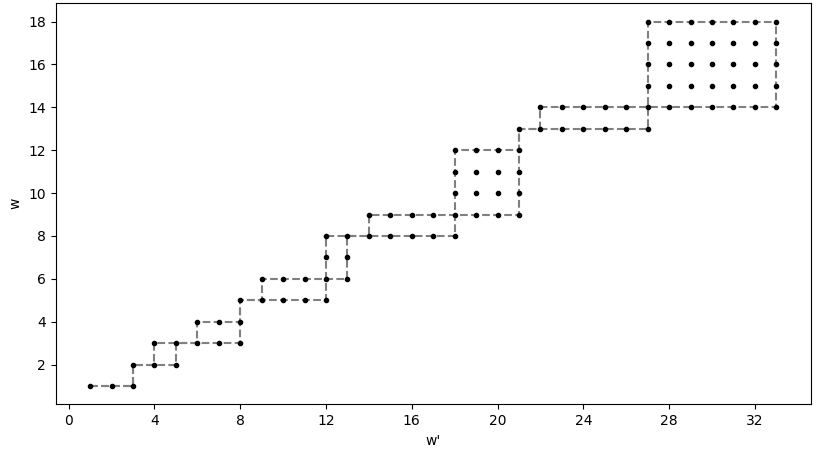
\includegraphics[scale=0.8]{w-n.png}


\vspace{1cm}
\begin{lemma}[Joint]
	Define the function $\eta : (\min\{s, t\}, \infty) \to \mathbb{Z}^+$
	\begin{align*}
	\eta(x) = \begin{cases} 1  &(\min\{s, t\}<x\le s+t)\\
	 \eta(x-s) + \eta(x-t)  &(x> s+t)
	\end{cases}
	\end{align*}
	This function is like stair cases, and has the form
	\begin{align*}
	\eta(x) = \begin{cases} \eta_1  &(\min\{s, t\}<x\le x_1)\\
	\eta_2  &(x_1<x\le x_2)\\
	\eta_3  &(x_2<x\le x_3)\\
	\eta_4  &(x_3<x\le x_4)\\
	\cdots
	\end{cases}
	\end{align*}
	where $\eta_1 = 1$,  $x_1 = s+t$ and the function is non-decreasing. It defines the ``joint sequence" $\{\eta_k\}_{k=1}^{\infty}$ that's strictly increasing
	\[
	\eta_1 < \eta_2 < \eta_3 < \eta_4 < \dots
	\]
	
	We call a tuple $(x_k, \eta_k\nearrow\eta_{k+1})$ a ``jump point". Each jump point is related to $E(n)$ in the range $n \in [\eta_k, \eta_{k+1})$. For $\eta_k \le n < \eta_{k+1}$
	\begin{align*}
	\Delta E_{s,t}(n) &= x_k\\
	w^{\min}_{s,t}(n) &= \max\{\eta(x_k-t),\, \eta(x_{k+1}-t) + n -\eta_{k+1}\}\quad(n\geq 2)	\\
	w^{\max}_{s,t}(n) &= \min\{\eta(x_{k+1}-t),\,\eta(x_k-t) + n -\eta_k \} \quad(n\geq 2)
	\end{align*}
	Specifically
	\[
	w_{s,t}(\eta_k) = \{\eta(x_k-t)\}\quad(\eta_k\geq 2)
	\]
	In other words, a jump point corresponds to a bead in $w(n)$. The bead may be degenerated to a thin straight line in some cases.
\end{lemma}
\begin{proof}
		Proof by induction
	\paragraph{Base case}
	The first jump point is $(x_1, \eta_1\nearrow\eta_2) = (s+t, 1\nearrow2)$, which corresponds to $n = 1$. We have shown that $\Delta E(1) = s + t$ so the base case is satisfied.
	
	\paragraph{Inductive step} A jump point $(x_k, \eta_k\nearrow\eta_{k+1})$, is related to two previous ``probable jump point" $(x_k-s, S\nearrow_?S')$ and $(x_k-t, T\nearrow_?T')$, with the following relation
	\begin{align*}
	S &= \eta(x_k-s)\\
	T &= \eta(x_k-t)\\
	S' &= \eta(x_{k+1}-s)\\
	T' &= \eta(x_{k+1}-t)\\
	S + T &= \eta_k \\
	S' + T' &= \eta_{k+1}
	\end{align*}
	At least one of the two probable jump points $x_k-s$, $x_k-t$ must be a real jump point (otherwise $x_k$ wouldn't be a jump point). And then we have the following inequalities 
	\begin{align*}
	\Delta E(S) &\ge x_k - s &(\text{Equal when $x_k-s$ is a jump point}) \\
	\Delta E(T) &\ge x_k - t &(\text{Equal when $x_k-t$ is a jump point}) \\
	\Delta E(S+1) &\ge \Delta E(S) \ge x_k - s  &(\text{Due to convexity of $E$})\\
	\Delta E(T+1) &\ge \Delta E(T) \ge x_k - t \\
	\Delta E(S-1) &< x_k - s &(\text{if $S\ge 2$})\\
	\Delta E(T-1) &< x_k - t &(\text{if $T\ge 2$})\\
	\end{align*}
	Let's look at the starting point of the current interval $E(\eta_k)$ around $w = T$. The differential $\Delta_w D$ are
	\begin{align*}
	\Delta_w D^{T - 1}(\eta_k) &= \Delta E(T-1) - \Delta E(\eta_k - T) + t - s\\
	&= \Delta E(T-1) - \Delta E(S) + t - s\\
	&< (x_k - t) - (x_k - s) + t - s = 0
	\end{align*}
	\begin{align*}
	\Delta_w D^{T }(\eta_k) &= \Delta E(T) - \Delta E(\eta_k - T - 1) + t - s\\
	&= \Delta E(T) - \Delta E(S - 1) + t - s\\
	&> (x_k - t) - (x_k - s) + t - s = 0
	\end{align*}
	Either of them might not exist for $T = 1$ or $T = \eta_k - 1$, but it doesn't affect the arguments. Because of convexity of $D^w$, this means 
	\[
	w(\eta_k) = \{T\} = \{\eta(x_k-t)\}
	\]
	and
	\[
	E(\eta_k) = E(T) + E(S) + T t + S s
	\]
	We can use the same argument for the last point of the current interval and get
	\[
	w(\eta_{k+1}) = \{T'\}
	\]
	\[
	E(\eta_{k+1}) = E(T') + E(S') + T' t + S' s
	\]
	The total difference between the two end points is
	\begin{align*}
	E(\eta_{k+1}) - E(\eta_k) &= E(T') - E(T) + E(S') - E(S) + (T'-T)t + (S'-S)s\\
	&= (T'-T)(x_k-t) + (S'-S)(x_k-s) + (T'-T)t + (S'-S)s \quad \\
	&(\text{This is true regardless whether the $x_k-t$ or $x_k-s$ is real jump points})\\
	&=(T'-T + S' - S)x_k\\
	&=(\eta_{k+1} -\eta_k)x_k
	\end{align*}
	If $\eta_{k+1} -\eta_k = 1$, then 
	\[
	E(\eta_{k+1}) - E(\eta_k) = \Delta E(\eta_k) = x_k
	\]
	and the current interval is proved. Otherwise, let's look at $E(\eta_k +1)$ around $w = T$ and $w = T+1$. The differential $\Delta_w D$ are
	\begin{align*}
	\Delta_w D^{T - 1}(\eta_k+1) &= \Delta E(T-1) - \Delta E(\eta_k - T + 1) + t - s\\
	&=\Delta E(T-1) - \Delta E(S + 1) + t - s\\
	&< (x_k - t) - (x_k -s) + t -s = 0
	\end{align*}
	\begin{align*}
	\Delta_w D^{T + 1}(\eta_k+1) &= \Delta E(T+1) - \Delta E(\eta_k - T - 1) + t - s\\
	&=\Delta E(T+1) - \Delta E(S - 1) + t - s\\
	&> (x_k - t) - (x_k -s) + t -s = 0
	\end{align*}
	Again, either of them might not exist, but anyway, due to convexity, the optimizer is among $w\in\{T, T+1\}$ (or potentially both). Their $D^w(\eta_k+1)$ are 
	\begin{align*}
	D^T(\eta_k+1) &= E(T) + E(\eta_k+1-T) +Tt +(\eta_k+1-T)s \\
	&= E(T) + E(S+1) +Tt +(S+1)s\\
	&= E(T) + E(S) + \Delta E(S) +Tt +(S+1)s\\
	&= E(\eta_k) + \Delta E(S) +s \\
	&\geq E(\eta_k) + x_k \quad (\text{equality holds when $x_k-s$ is a jump point})
	\end{align*}
	\begin{align*}
	D^{T+1}(\eta_k+1) &= E(T+1) + E(\eta_k-T) +(T+1)t +(\eta_k-T)s \\
	&= E(T+1) + E(S) +(T+1)t +Ss \\
	&= E(T) + \Delta E(T)+ E(S) +  (T+1)t +Ss\\
	&= E(\eta_k) + \Delta E(T) +t \\
	&\geq E(\eta_k) + x_k \quad (\text{equality holds when $x_k-t$ is a jump point})
	\end{align*}
	Because at least one of the equality holds, we have
	\[
	E(\eta_k+1) =  E(\eta_k) + x_k
	\]
	The choice of $w$ among $\{T, T+1\}$ depends on which are jump points
	\begin{itemize}
		\item $x_k-s$ is a jump point $\iff T \in w(\eta_k+1)$ 
		\item $x_k-t$ is a jump point $\iff T+1 \in w(\eta_k+1)$ 
	\end{itemize}
	Then $\Delta E(\eta_k)$ would be 
	\begin{align*}
	\Delta E(\eta_k) &= E(\eta_k+1) - E(\eta_k) \\
	&= x_k 
	\end{align*}
	Remember $E(\eta_{k+1}) - E(\eta_k) = (\eta_{k+1} -\eta_k)x_k$, then we have 
	\begin{align*}
	(\eta_{k+1} -\eta_k)x_k &= E(\eta_{k+1}) - E(\eta_k) \\
	&= \Delta E(\eta_k) + \Delta E(\eta_k + 1) +\dots+\Delta E(\eta_{k+1} - 1) \\
	&\geq  \Delta E(\eta_k) + \Delta E(\eta_k) +\dots+\Delta E(\eta_k) \\
	&\geq (\eta_{k+1} -\eta_k)x_k
	\end{align*}
	This equality must holds, so this locks all $\Delta E(n) = x_k$ for $\eta_{k} \leq n < \eta_{k+1}$, and this proves the formula for $\Delta E(n)$.
	
	As for the values of $w(n)$ in between, we have three cases 
	\begin{itemize}
		\item If both $x_k-s$ and $x_k-t$ are jump points, then we have $w(\eta_k +1) =\{T, T+1\}$, and $E(n)$ is linear for $n \in [S, S']$ and $n \in [T, T']$. We have shown that $w(n)$ will form a parallelogram that satisfy the formula.
		\item If $x_k-s$ is not a jump point, then we have the following equations
		\begin{align*}
		S &= S'\\
		w(\eta_{k}) &= \{T\}\\
		w(\eta_{k+1}) &= \{T'\} = \{T+\eta_{k+1} - \eta_k\}
		\end{align*}
		The two end points form a slope of 1. Because of $w$-Lipschitz continuity, this forces all $w(n)$ to be on the thin line $w(\eta_{k} + a) = \{T+a\}$.
		\item If $x_k-t$ is not a jump point, then we have the following equations 
		\begin{align*}
		T &= T'\\
		w(\eta_{k}) &= \{T\}\\
		w(\eta_{k+1}) &= \{T'\} = \{T\}
		\end{align*}
		The two end points are on the same level. Because of $w$-Lipschitz continuity, this forces all $w(n)$ to be on the same level.
	\end{itemize}
	In summary, we have proved the formula for $w(n)$
	

\end{proof}

\paragraph{Remark}

Although we defined $\eta(n)$ on all real numbers in $(\min\{s, t\}, \infty)$, not all of them are important. It is easy to see that jump points $x_k$ can only be in the following subsets
\begin{itemize}
	\item for $s/t\in\mathbb{Q}$, $x_k \in \gcd(s,t)\mathbb{Z}$. Specifically, if $s$ and $t$ are integers, $x_k\in\mathbb{Z}$. We will discuss this in the next property.
	\item for $s/t\notin\mathbb{Q}$, $x_k \in s\mathbb{Z} + t\mathbb{Z}$, a subset of an algebraic number field with bases $\{s, t\}$
\end{itemize}
Another way to put this is that the jump point sequence $\{x_k\}_{k=1}^{\infty}$ is all elements in ascending order from the set
\[
	J_{s,t} = \{ps+qt\ |\  p \in \mathbb{Z}^+, q \in \mathbb{Z}^+\}
\]

The function $\Delta E(n)$ is, in some sense, the inverse function of $\eta(x)$. Of course, $\eta(x)$ is not injective, so we take the inverse in this way: for each flat line in $\eta(n)$ which becomes vertical in the inverse, we take the highest point as the inverse function value. We also connects the vertical jumps in $\eta(n)$, which becomes flat in the inverse. The $\Delta E(n)$ function, defined over $n \in [1, \infty)$ (for real numbers) is
\begin{align*}
\Delta E(n) = \begin{cases}
x_1 & (1 = \eta_1 \le n < \eta_2) \\
x_2 & (\eta_2 \le n < \eta_3) \\
x_3 & (\eta_3 \le n < \eta_4) \\
\dots
\end{cases}
\end{align*}
and the function $E(n)$ is the integral 
\begin{align*}
E(n) &= \int_1^n \Delta E(m)\, dm \\
 &= \left(\sum_{k = 1}^{h-1} x_k (\eta_{k+1} - \eta_k)\right) + x_{h} (n - \eta_{h}) \quad (\eta_{h} \le n < \eta_{h+1}) \\
 &= n x_h - \left(\eta_1 \min\{s, t\} + \int_{\min\{s, t\}}^{x_h} \eta(x)\, dx\right)\\
 &= n x_h  - \left(\eta_1 x_1 + \sum_{k=2}^{h} \eta_k (x_{h} - x_{h-1})\right)
\end{align*}
This also conforms to a natural extension of $E(n)$ for real number $n$: it is linear interpolation between nearest integer points.

Below is the graph of $n = \eta(x)$ and $x = \Delta E(n)$ for $s = \sqrt{2}, t = \sqrt{3}$.

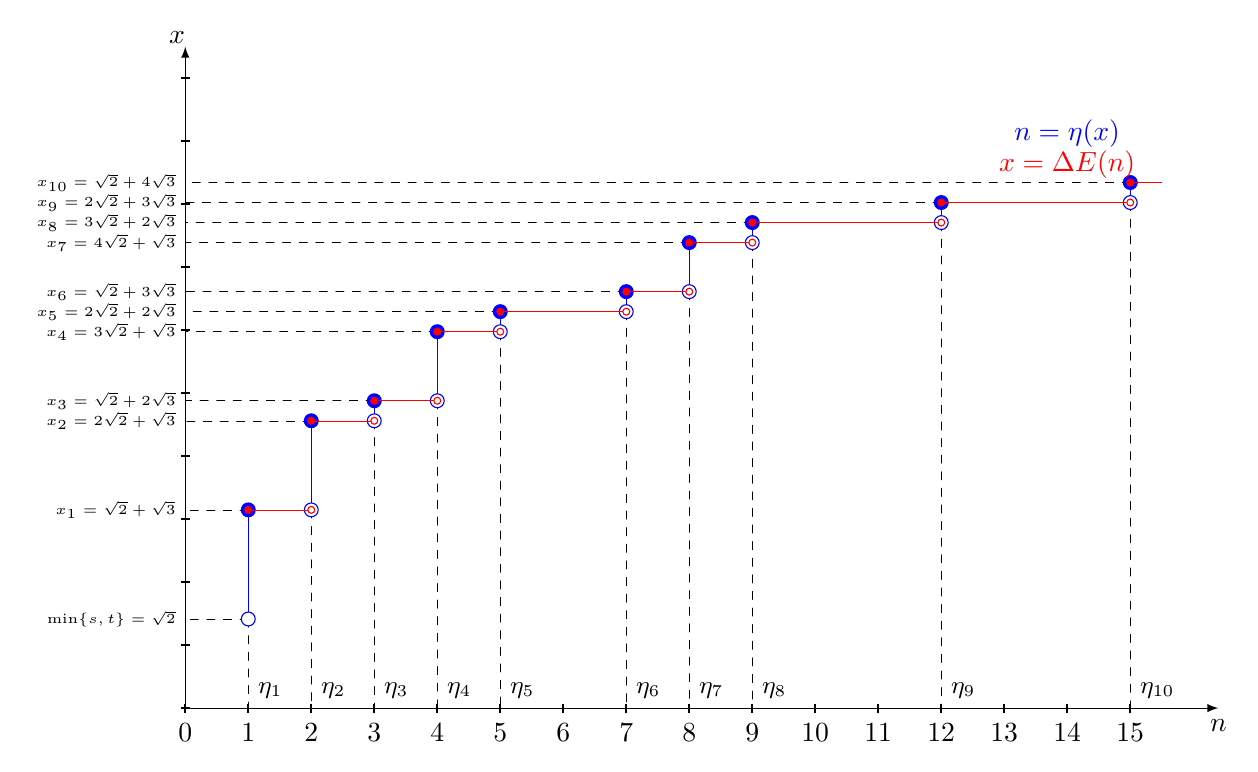
\begin{tikzpicture}[yscale=0.8,xscale=0.8]
\tkzInit[xmin=0,ymin=0,xmax=15.9,ymax=10,xstep=1,ystep=1]
\tkzDrawX[label={$n$}]
\tkzLabelX[step=1]
\tkzDrawY[label={$x$},above]
%\tkzLabelY[step=1]
\tkzDefPoint( 1, 3.1462643699419726){p0} 
\tkzDefPoint( 2, 4.5604779323150675){p1} 
\tkzDefPoint( 3, 4.878315177510849 ){p2}
\tkzDefPoint( 4, 5.974691494688162 ){p3}
\tkzDefPoint( 5, 6.292528739883945 ){p4}
\tkzDefPoint( 7, 6.610365985079727 ){p5}
\tkzDefPoint( 8, 7.388905057061258 ){p6}
\tkzDefPoint( 9, 7.70674230225704  ){p7}
\tkzDefPoint(12, 8.024579547452822 ){p8}
\tkzDefPoint(15, 8.342416792648605 ){p9}

\tkzDefPoint(0, 1.4142135623730950){pp} 
\tkzDefPoint(0, 3.1462643699419726){pp0} 
\tkzDefPoint(0, 4.5604779323150675){pp1} 
\tkzDefPoint(0, 4.878315177510849 ){pp2}
\tkzDefPoint(0, 5.974691494688162 ){pp3}
\tkzDefPoint(0, 6.292528739883945 ){pp4}
\tkzDefPoint(0, 6.610365985079727 ){pp5}
\tkzDefPoint(0, 7.388905057061258 ){pp6}
\tkzDefPoint(0, 7.70674230225704  ){pp7}
\tkzDefPoint(0, 8.024579547452822 ){pp8}
\tkzDefPoint(0, 8.342416792648605 ){pp9}

\tkzDefPoint( 1, 1.4142135623730950){q}
\tkzDefPoint( 2, 3.1462643699419726){q0} 
\tkzDefPoint( 3, 4.5604779323150675){q1} 
\tkzDefPoint( 4, 4.878315177510849 ){q2}
\tkzDefPoint( 5, 5.974691494688162 ){q3}
\tkzDefPoint( 7, 6.292528739883945 ){q4}
\tkzDefPoint( 8, 6.610365985079727 ){q5}
\tkzDefPoint( 9, 7.388905057061258 ){q6}
\tkzDefPoint(12, 7.70674230225704  ){q7}
\tkzDefPoint(15, 8.024579547452822 ){q8}
\tkzDefPoint(15.5, 8.342416792648605 ){qe}

\tkzDefPoint( 1, 0){qq}
\tkzDefPoint( 2, 0){qq0} 
\tkzDefPoint( 3, 0){qq1} 
\tkzDefPoint( 4, 0){qq2}
\tkzDefPoint( 5, 0){qq3}
\tkzDefPoint( 7, 0){qq4}
\tkzDefPoint( 8, 0){qq5}
\tkzDefPoint( 9, 0){qq6}
\tkzDefPoint(12, 0){qq7}
\tkzDefPoint(15, 0){qq8}

\tkzDrawSegments[style=dashed](q,pp p0,pp0 p1,pp1 p2,pp2 p3,pp3 p4,pp4 p5,pp5 p6,pp6 p7,pp7 p8,pp8 p9,pp9)
\tkzDrawSegments[style=dashed](q,qq q0,qq0 q1,qq1 q2,qq2 q3,qq3 q4,qq4 q5,qq5 q6,qq6 q7,qq7 q8,qq8)

\tkzDrawSegments[color=blue](q,p0 q0,p1 q1,p2 q2,p3 q3,p4 q4,p5 q5,p6 q6,p7 q7,p8 q8,p9)
\tkzDrawPoints[size=5,color=blue](p0,p1,p2,p3,p4,p5,p6,p7,p8,p9)
\tkzDrawPoints[size=5,color=blue,fill=white](q,q0,q1,q2,q3,q4,q5,q6,q7,q8)

\tkzDrawSegments[color=red](p0,q0 p1,q1 p2,q2 p3,q3 p4,q4 p5,q5 p6,q6 p7,q7 p8,q8 p9,qe)
\tkzDrawPoints[size=2.5,color=red](p0,p1,p2,p3,p4,p5,p6,p7,p8,p9)
\tkzDrawPoints[size=2.5,color=red,fill=white](q0,q1,q2,q3,q4,q5,q6,q7,q8)


\tkzLabelPoint[color=blue]({14,9.5}){$n = \eta(x)$}
\tkzLabelPoint[color=red]({14,9}){$x = \Delta E(n)$}

\tkzLabelPoint[left](pp){\tiny $\min\{s,t\}=\sqrt{2}$}
\tkzLabelPoint[left](pp0){\tiny $x_1=\sqrt{2}+\sqrt{3}$}
\tkzLabelPoint[left](pp1){\tiny $x_2=2\sqrt{2}+\sqrt{3}$}
\tkzLabelPoint[left](pp2){\tiny $x_3=\sqrt{2}+2\sqrt{3}$}
\tkzLabelPoint[left](pp3){\tiny $x_4=3\sqrt{2}+\sqrt{3}$}
\tkzLabelPoint[left](pp4){\tiny $x_5=2\sqrt{2}+2\sqrt{3}$}
\tkzLabelPoint[left](pp5){\tiny $x_6=\sqrt{2}+3\sqrt{3}$}
\tkzLabelPoint[left](pp6){\tiny $x_7=4\sqrt{2}+\sqrt{3}$}
\tkzLabelPoint[left](pp7){\tiny $x_8=3\sqrt{2}+2\sqrt{3}$}
\tkzLabelPoint[left](pp8){\tiny $x_9=2\sqrt{2}+3\sqrt{3}$}
\tkzLabelPoint[left](pp9){\tiny $x_{10}=\sqrt{2}+4\sqrt{3}$}

\tkzLabelPoint[above right](qq){\small $\eta_1$}
\tkzLabelPoint[above right](qq0){\small $\eta_2$}
\tkzLabelPoint[above right](qq1){\small $\eta_3$}
\tkzLabelPoint[above right](qq2){\small $\eta_4$}
\tkzLabelPoint[above right](qq3){\small $\eta_5$}
\tkzLabelPoint[above right](qq4){\small $\eta_6$}
\tkzLabelPoint[above right](qq5){\small $\eta_7$}
\tkzLabelPoint[above right](qq6){\small $\eta_8$}
\tkzLabelPoint[above right](qq7){\small $\eta_9$}
\tkzLabelPoint[above right](qq8){\small $\eta_{10}$}

\end{tikzpicture}

\vspace{1cm}

Additionally, we can define the following ``jump height function" $\delta: (\min\{s,t\},\infty)\to\mathbb{Z}^{0+}$, which is the length of red segments in the graph above
\begin{align*}
\delta(x) = \eta(x^+) - \eta(x^-) =\begin{cases}
\eta_{i+1} - \eta_{i} & (x = x_i)\\
0 & (\text{otherwise})\\
\end{cases}
\end{align*}
which can also be expressed with the recursive formula
\begin{align*}
\delta(x) = \begin{cases}
0 & (x \in (\min\{s, t\}, s + t))\\
1 & (x = s+t)\\
\delta(x-s)+ \delta(x-t) & (x\in(s+t,\infty))
\end{cases}
\end{align*}
For $s/t\notin\mathbb{Q}$, the jump point set $J_{s,t}$ has one-to-one correspondence to positive integer pairs $(p,q)\in(\mathbb{Z}^+)^2$. This means, for $(p,q)\in(\mathbb{Z}^{0+})^2 / \{(0,0), (0,1), (1,0)\}$
\begin{align*}
\delta(ps+qt) = \begin{cases}
 0 & (p= 0 \text{ or } q = 0) \\
 1 & (p = q = 1) \\
 \delta((p-1)s+qt) + \delta(ps+(q-1)t) & (\text{otherwise})
\end{cases}
\end{align*}
It is easy to see $\delta$ forms a Pascal's triangle over $(p,q)\in(\mathbb{Z}^+)^2$
\[
	\delta(ps+qt) = \binom{p+q-2}{q-1} = \frac{(p+q-2)!}{(p-1)!(q-1)!}
\]
This can be further generalized to make it also work for $s/t\in\mathbb{Q}$ as 
\[
	\delta(x) = \sum_{(p,q)\in(\mathbb{Z}^+)^2}^{ps+qt = x} \frac{(p+q-2)!}{(p-1)!(q-1)!}
\]
To see how this works for rational $s/t$, we can still map $x$ to integer pair $(p, q)$ - except this time a line of many $(p, q)$ correspond to the same $x$. For the first jump point $x = s + t$, all $(p, q)$ such that $ps + qt = s + t$ will have corresponding $\delta = 1$. This is equivalent to ``seeding" Pascal's triangles at many places, so the resulting $\delta$ value everywhere should be the sum of all these Pascal's triangles.

This gives rise to an alternative way to express $\eta(x)$
\[
	\eta(x) = 1 + \sum_{x_i < x} \delta(x_i) = 1 + \sum_{(p,q)\in(\mathbb{Z}^+)^2}^{ps+qt < x} \frac{(p+q-2)!}{(p-1)!(q-1)!}
\]

\vspace{1cm}
\begin{lemma}[Fibonacci]
	Given positive integer $s$ and $t$, define the non-decreasing ``generalized Fibonacci sequence" $\{n_i\}_{i=\min\{s,t\}+1}^\infty$ as
	\[
	n_{\min\{s,t\}+1} = \dots = n_{s + t} = 1
	\]
	\[
	n_{i} = n_{i - s} + n_{i - t} , \quad i > s + t
	\]
	then we have, when $n_i \neq n_{i+1}$, for $n_i \le n < n_{i+1}$
	\begin{align*}
	\Delta E_{s,t}(n) &= i\\
	w^{\min}_{s,t}(n) &= \max\{n_{i - t},\, n_{i +1 - t} + n - n_{i+1}\}\quad(n\geq 2)	\\
	w^{\max}_{s,t}(n) &= \min\{n_{i +1 - t},\,n_{i - t} + n - n_{i} \} \quad(n\geq 2)
	\end{align*}
\end{lemma}
\begin{proof}
	We can construct $\{n_i\}_{i=\min\{s,t\}+1}^{\infty}$ from $\eta(x)$ as
	\[
	n_i = \eta(i)
	\]
	and one can easily verify that this satisfies the recurrence relation of both $\eta(x)$ and $\{n_i\}_{i}$. And for every $n_i \neq n_{i+1}$, there is a jump point at $(i,n_i\nearrow n_{i+1})$, and we can derive the $\Delta E_{s,t}(n)$ and $w_{s,t}(n)$ formula for integer case from the previous property.
	
\end{proof}	

\paragraph{Remark}

This property provides a way to recursively generate linear segments for $E(n)$ when $s$ and $t$ are integers (and by extension due to homogeneity, whenever $s/t$ is rational). For example, for $s = t = 1$ (balanced bisection), we have the following
\begin{align*}
\Delta E_{1,1}(1) &= 2 \\
\Delta E_{1,1}(2) = \Delta E_{1,1}(3) &= 3\\
\Delta E_{1,1}(4) =\dots = \Delta E_{1,1}(7) &= 4\\
\Delta E_{1,1}(2^{i-2}) =\dots = \Delta E_{1,1}(2^{i-1}-1) &= i
\end{align*}
This forms a nice geometric progression.

Similarly, for $s = 1$ and $t = 2$, we have 
\begin{align*}
\Delta E_{1,2}(1) &= 3 \\
\Delta E_{1,2}(2) &= 4\\
\Delta E_{1,2}(3)  = \Delta E_{1,2}(4) &= 5\\
\Delta E_{1,2}(5) =\dots = \Delta E_{1,2}(7) &= 6\\
\Delta E_{1,2}(8) =\dots = \Delta E_{1,2}(12) &= 7\\
\Delta E_{1,2}(\phi_{i -1}) =\dots = \Delta E_{1,2}(\phi_{i} - 1) &= i
\end{align*}
where $\phi_i$ is the $i$th Fibonacci number.
	
\vspace{1cm}
\begin{lemma}[$s,t$-concavity]
Fixing $n$ and $s$, $E_{s,t}(n)$ as a function of $t$ is concave 
\end{lemma}
\begin{proof}
Proof by induction. The base case $E_{s,t}(1) = 0$ is concave over $t$. In the recursive equation, all the summation components are concave, and the minimal of concave functions is still a concave function.
\end{proof}

\vspace{1cm}
\begin{lemma}[$s,t$-linearity]
Fixing $n$ and $s$, $E_{s,t}(n)$ is a piecewise linear function of $t$. The nodes are always at rational points.
\end{lemma}
\begin{proof}
	This can be proved by induction. Omitted.
\end{proof}

\paragraph{Remark}
With this property, we can graph the function with a series of segments. For example, the graph of $E_{1,t}(29)$ over $t\in[0,1]$ is 

\vspace{0.5cm}
	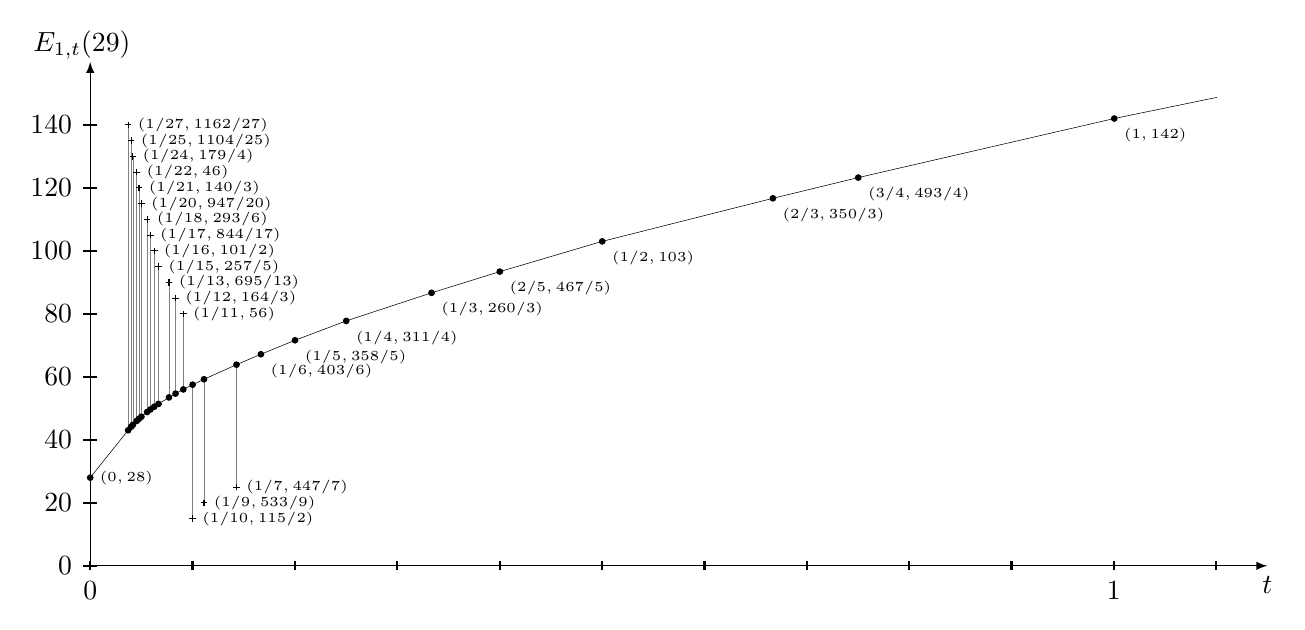
\begin{tikzpicture}[yscale=0.8,xscale=1.3]
	\tkzInit[xmin=0,ymin=0,xmax=1.1,ymax=150,xstep=0.1,ystep=20]
	\tkzDrawX[label={$t$}]
	\tkzLabelX[step=1]
	\tkzDrawY[label={$E_{1,t}(29)$},above]
	\tkzLabelY[step=10]
	
\tkzDefPoint(0,28){p0}
\tkzDefPoint(1/27,1162/27){p1} \tkzDrawSegment(p0,p1)
\tkzDefPoint(1/25,1104/25){p2} \tkzDrawSegment(p1,p2)
\tkzDefPoint(1/24,179/4){p3} \tkzDrawSegment(p2,p3)
\tkzDefPoint(1/22,46){p4} \tkzDrawSegment(p3,p4)
\tkzDefPoint(1/21,140/3){p5} \tkzDrawSegment(p4,p5)
\tkzDefPoint(1/20,947/20){p6} \tkzDrawSegment(p5,p6)
\tkzDefPoint(1/18,293/6){p7} \tkzDrawSegment(p6,p7)
\tkzDefPoint(1/17,844/17){p8} \tkzDrawSegment(p7,p8)
\tkzDefPoint(1/16,101/2){p9} \tkzDrawSegment(p8,p9)
\tkzDefPoint(1/15,257/5){p10} \tkzDrawSegment(p9,p10)
\tkzDefPoint(1/13,695/13){p11} \tkzDrawSegment(p10,p11)
\tkzDefPoint(1/12,164/3){p12} \tkzDrawSegment(p11,p12)
\tkzDefPoint(1/11,56){p13} \tkzDrawSegment(p12,p13)
\tkzDefPoint(1/10,115/2){p14} \tkzDrawSegment(p13,p14)
\tkzDefPoint(1/9,533/9){p15} \tkzDrawSegment(p14,p15)
\tkzDefPoint(1/7,447/7){p16} \tkzDrawSegment(p15,p16)
\tkzDefPoint(1/6,403/6){p17} \tkzDrawSegment(p16,p17)
\tkzDefPoint(1/5,358/5){p18} \tkzDrawSegment(p17,p18)
\tkzDefPoint(1/4,311/4){p19} \tkzDrawSegment(p18,p19)
\tkzDefPoint(1/3,260/3){p20} \tkzDrawSegment(p19,p20)
\tkzDefPoint(2/5,467/5){p21} \tkzDrawSegment(p20,p21)
\tkzDefPoint(1/2,103){p22} \tkzDrawSegment(p21,p22)
\tkzDefPoint(2/3,350/3){p23} \tkzDrawSegment(p22,p23)
\tkzDefPoint(3/4,493/4){p24} \tkzDrawSegment(p23,p24)
\tkzDefPoint(1,142){p25} \tkzDrawSegment(p24,p25)
\tkzDefPoint(1.1,148.7){p26} \tkzDrawSegment(p25,p26)
\tkzLabelPoint[right](p0){\tiny $(0,28)$}
\tkzDefPoint(1/27,140){p1l}\tkzDrawSegment[color=gray](p1,p1l)\tkzDrawPoints[shape=cross](p1l)\tkzLabelPoint[right](p1l){\tiny $(1/27,1162/27)$}
\tkzDefPoint(1/25,135){p2l}\tkzDrawSegment[color=gray](p2,p2l)\tkzDrawPoints[shape=cross](p2l)\tkzLabelPoint[right](p2l){\tiny $(1/25,1104/25)$}
\tkzDefPoint(1/24,130){p3l}\tkzDrawSegment[color=gray](p3,p3l)\tkzDrawPoints[shape=cross](p3l)\tkzLabelPoint[right](p3l){\tiny $(1/24,179/4)$}
\tkzDefPoint(1/22,125){p4l}\tkzDrawSegment[color=gray](p4,p4l)\tkzDrawPoints[shape=cross](p4l)\tkzLabelPoint[right](p4l){\tiny $(1/22,46)$}
\tkzDefPoint(1/21,120){p5l}\tkzDrawSegment[color=gray](p5,p5l)\tkzDrawPoints[shape=cross](p5l)\tkzLabelPoint[right](p5l){\tiny $(1/21,140/3)$}
\tkzDefPoint(1/20,115){p6l}\tkzDrawSegment[color=gray](p6,p6l)\tkzDrawPoints[shape=cross](p6l)\tkzLabelPoint[right](p6l){\tiny $(1/20,947/20)$}
\tkzDefPoint(1/18,110){p7l}\tkzDrawSegment[color=gray](p7,p7l)\tkzDrawPoints[shape=cross](p7l)\tkzLabelPoint[right](p7l){\tiny $(1/18,293/6)$}
\tkzDefPoint(1/17,105){p8l}\tkzDrawSegment[color=gray](p8,p8l)\tkzDrawPoints[shape=cross](p8l)\tkzLabelPoint[right](p8l){\tiny $(1/17,844/17)$}
\tkzDefPoint(1/16,100){p9l}\tkzDrawSegment[color=gray](p9,p9l)\tkzDrawPoints[shape=cross](p9l)\tkzLabelPoint[right](p9l){\tiny $(1/16,101/2)$}
\tkzDefPoint(1/15,95){p10l}\tkzDrawSegment[color=gray](p10,p10l)\tkzDrawPoints[shape=cross](p10l)\tkzLabelPoint[right](p10l){\tiny $(1/15,257/5)$}
\tkzDefPoint(1/13,90){p11l}\tkzDrawSegment[color=gray](p11,p11l)\tkzDrawPoints[shape=cross](p11l)\tkzLabelPoint[right](p11l){\tiny $(1/13,695/13)$}
\tkzDefPoint(1/12,85){p12l}\tkzDrawSegment[color=gray](p12,p12l)\tkzDrawPoints[shape=cross](p12l)\tkzLabelPoint[right](p12l){\tiny $(1/12,164/3)$}
\tkzDefPoint(1/11,80){p13l}\tkzDrawSegment[color=gray](p13,p13l)\tkzDrawPoints[shape=cross](p13l)\tkzLabelPoint[right](p13l){\tiny $(1/11,56)$}
\tkzDefPoint(1/10,15){p14l}\tkzDrawSegment[color=gray](p14,p14l)\tkzDrawPoints[shape=cross](p14l)\tkzLabelPoint[right](p14l){\tiny $(1/10,115/2)$}
\tkzDefPoint(1/9,20){p15l}\tkzDrawSegment[color=gray](p15,p15l)\tkzDrawPoints[shape=cross](p15l)\tkzLabelPoint[right](p15l){\tiny $(1/9,533/9)$}
\tkzDefPoint(1/7,25){p16l}\tkzDrawSegment[color=gray](p16,p16l)\tkzDrawPoints[shape=cross](p16l)\tkzLabelPoint[right](p16l){\tiny $(1/7,447/7)$}
\tkzLabelPoint[right,anchor=north west](p17){\tiny $(1/6,403/6)$}
\tkzLabelPoint[right,anchor=north west](p18){\tiny $(1/5,358/5)$}
\tkzLabelPoint[right,anchor=north west](p19){\tiny $(1/4,311/4)$}
\tkzLabelPoint[right,anchor=north west](p20){\tiny $(1/3,260/3)$}
\tkzLabelPoint[right,anchor=north west](p21){\tiny $(2/5,467/5)$}
\tkzLabelPoint[right,anchor=north west](p22){\tiny $(1/2,103)$}
\tkzLabelPoint[right,anchor=north west](p23){\tiny $(2/3,350/3)$}
\tkzLabelPoint[right,anchor=north west](p24){\tiny $(3/4,493/4)$}
\tkzLabelPoint[right,anchor=north west](p25){\tiny $(1,142)$}
\tkzDrawPoints(p0,p1,p2,p3,p4,p5,p6,p7,p8,p9,p10,p11,p12,p13,p14,p15,p16,p17,p18,p19,p20,p21,p22,p23,p24,p25)

	\end{tikzpicture}

We omitted the graph beyond $t=1$, but remember that it can be derived by $E_{1,t}(n) = t\cdot E_{1,1/t}(n)$ due to symmetry and homogeneity.

It can be seen from the graph that nodes are most at unit fractions $t = 1/p$, but there are also a few nodes at non-unit fractions close to $t=1$.
\vspace{1cm}
\begin{lemma}[$s,t$-range]
	Fixing $n$ and $s$, $w_{s,t}(n)$ is a ``piecewise constant" function. Over a single segment of the piecewise function $E_{s,t}(n)$, the same set of $w$ is chosen. However, exactly at a node of piecewise function $E_{s,t}(n)$, $w_{s,t}(n)$ can take a unique value that's not equal to either the one of the left segment or the one of the right segment.
\end{lemma}
\begin{proof}
	Remember that $E_{s,t}(n)$ calculated by taking the $t$-pointwise minimum of a sequence of piecewise linear, convex functions $D^w(t)$ indexed by $w$. If the pointwise minimum results in a simple linear function over a $t$-interval, it must be resulted from the same set of $w$. This is because, if any $D^w_{s,t}(n)$ tries to join or leave $E_{s,t}(n)$ midway in the interval, it must bend down due to convexity, and that would result in  $E_{s,t}(n) \le D^w_{s,t}(n)$ bending down as well, contradicting with the fact that $E_{s,t}(n)$ is a simple linear function in this interval. $D^w_{s,t}(n)$ can only join or leave at the nodes of $E_{s,t}(n)$
\end{proof}

\paragraph{Remark}

If we graph $w$ over $t$, we will get a series of ``blocks", separated by vertical lines (marked red) at the nodes of $E$ over $t$. For example, the graph of $w_{1,t}(29)$ over $t\in[0,1]$ is 

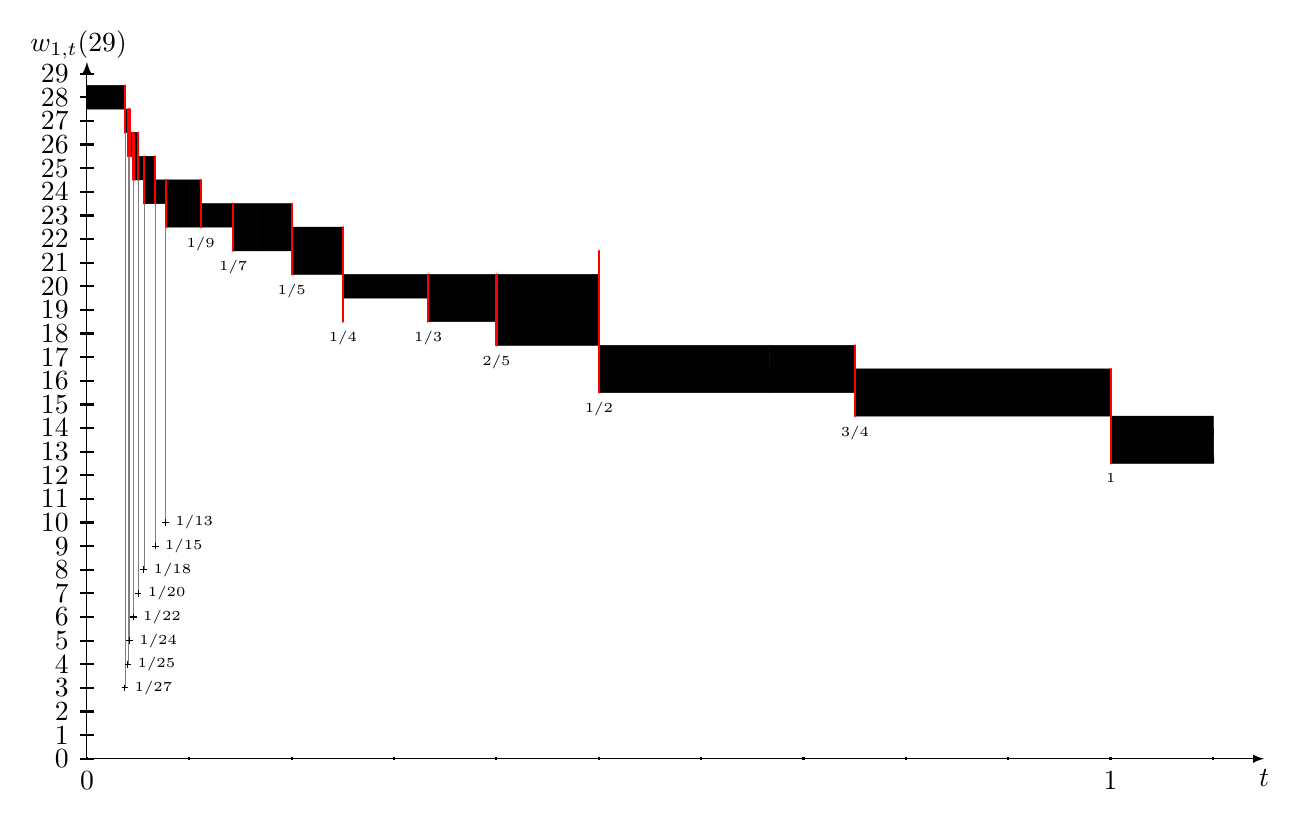
\begin{tikzpicture}[yscale=0.3,xscale=1.3]
\tkzInit[xmin=0,ymin=0,xmax=1.1,ymax=29,xstep=0.1,ystep=1]
\tkzDrawX[label={$t$}]
\tkzLabelX[step=1]
\tkzDrawY[label={$w_{1,t}(29)$},above]
\tkzLabelY[step=1]

\tkzDefPoint(0,27.5){A}\tkzDefPoint(1/27,28.5){C}\tkzDefRectangle(A,C)\tkzGetPoints{B}{D} \tkzDrawPolygon[fill=black](A,...,D)
\tkzDefPoint(1/27,26.5){A}\tkzDefPoint(1/25,27.5){C}\tkzDefRectangle(A,C)\tkzGetPoints{B}{D} \tkzDrawPolygon[fill=black](A,...,D)
\tkzDefPoint(1/25,25.5){A}\tkzDefPoint(1/24,27.5){C}\tkzDefRectangle(A,C)\tkzGetPoints{B}{D} \tkzDrawPolygon[fill=black](A,...,D)
\tkzDefPoint(1/24,25.5){A}\tkzDefPoint(1/22,26.5){C}\tkzDefRectangle(A,C)\tkzGetPoints{B}{D} \tkzDrawPolygon[fill=black](A,...,D)
\tkzDefPoint(1/22,24.5){A}\tkzDefPoint(1/21,26.5){C}\tkzDefRectangle(A,C)\tkzGetPoints{B}{D} \tkzDrawPolygon[fill=black](A,...,D)
\tkzDefPoint(1/21,24.5){A}\tkzDefPoint(1/20,26.5){C}\tkzDefRectangle(A,C)\tkzGetPoints{B}{D} \tkzDrawPolygon[fill=black](A,...,D)
\tkzDefPoint(1/20,24.5){A}\tkzDefPoint(1/18,25.5){C}\tkzDefRectangle(A,C)\tkzGetPoints{B}{D} \tkzDrawPolygon[fill=black](A,...,D)
\tkzDefPoint(1/18,23.5){A}\tkzDefPoint(1/17,25.5){C}\tkzDefRectangle(A,C)\tkzGetPoints{B}{D} \tkzDrawPolygon[fill=black](A,...,D)
\tkzDefPoint(1/17,23.5){A}\tkzDefPoint(1/16,25.5){C}\tkzDefRectangle(A,C)\tkzGetPoints{B}{D} \tkzDrawPolygon[fill=black](A,...,D)
\tkzDefPoint(1/16,23.5){A}\tkzDefPoint(1/15,25.5){C}\tkzDefRectangle(A,C)\tkzGetPoints{B}{D} \tkzDrawPolygon[fill=black](A,...,D)
\tkzDefPoint(1/15,23.5){A}\tkzDefPoint(1/13,24.5){C}\tkzDefRectangle(A,C)\tkzGetPoints{B}{D} \tkzDrawPolygon[fill=black](A,...,D)
\tkzDefPoint(1/13,22.5){A}\tkzDefPoint(1/12,24.5){C}\tkzDefRectangle(A,C)\tkzGetPoints{B}{D} \tkzDrawPolygon[fill=black](A,...,D)
\tkzDefPoint(1/12,22.5){A}\tkzDefPoint(1/11,24.5){C}\tkzDefRectangle(A,C)\tkzGetPoints{B}{D} \tkzDrawPolygon[fill=black](A,...,D)
\tkzDefPoint(1/11,22.5){A}\tkzDefPoint(1/10,24.5){C}\tkzDefRectangle(A,C)\tkzGetPoints{B}{D} \tkzDrawPolygon[fill=black](A,...,D)
\tkzDefPoint(1/10,22.5){A}\tkzDefPoint(1/9,24.5){C}\tkzDefRectangle(A,C)\tkzGetPoints{B}{D} \tkzDrawPolygon[fill=black](A,...,D)
\tkzDefPoint(1/9,22.5){A}\tkzDefPoint(1/7,23.5){C}\tkzDefRectangle(A,C)\tkzGetPoints{B}{D} \tkzDrawPolygon[fill=black](A,...,D)
\tkzDefPoint(1/7,21.5){A}\tkzDefPoint(1/6,23.5){C}\tkzDefRectangle(A,C)\tkzGetPoints{B}{D} \tkzDrawPolygon[fill=black](A,...,D)
\tkzDefPoint(1/6,21.5){A}\tkzDefPoint(1/5,23.5){C}\tkzDefRectangle(A,C)\tkzGetPoints{B}{D} \tkzDrawPolygon[fill=black](A,...,D)
\tkzDefPoint(1/5,20.5){A}\tkzDefPoint(1/4,22.5){C}\tkzDefRectangle(A,C)\tkzGetPoints{B}{D} \tkzDrawPolygon[fill=black](A,...,D)
\tkzDefPoint(1/4,19.5){A}\tkzDefPoint(1/3,20.5){C}\tkzDefRectangle(A,C)\tkzGetPoints{B}{D} \tkzDrawPolygon[fill=black](A,...,D)
\tkzDefPoint(1/3,18.5){A}\tkzDefPoint(2/5,20.5){C}\tkzDefRectangle(A,C)\tkzGetPoints{B}{D} \tkzDrawPolygon[fill=black](A,...,D)
\tkzDefPoint(2/5,17.5){A}\tkzDefPoint(1/2,20.5){C}\tkzDefRectangle(A,C)\tkzGetPoints{B}{D} \tkzDrawPolygon[fill=black](A,...,D)
\tkzDefPoint(1/2,15.5){A}\tkzDefPoint(2/3,17.5){C}\tkzDefRectangle(A,C)\tkzGetPoints{B}{D} \tkzDrawPolygon[fill=black](A,...,D)
\tkzDefPoint(2/3,15.5){A}\tkzDefPoint(3/4,17.5){C}\tkzDefRectangle(A,C)\tkzGetPoints{B}{D} \tkzDrawPolygon[fill=black](A,...,D)
\tkzDefPoint(3/4,14.5){A}\tkzDefPoint(1,16.5){C}\tkzDefRectangle(A,C)\tkzGetPoints{B}{D} \tkzDrawPolygon[fill=black](A,...,D)
\tkzDefPoint(1,12.5){A}\tkzDefPoint(1.1,14.5){C}\tkzDefRectangle(A,C)\tkzGetPoints{B}{D} \tkzDrawPolygon[fill=black](A,...,D)
\tkzDefPoint(1/27,26.5){A}\tkzDefPoint(1/27,28.5){B}\tkzDrawSegment[color=red,thick](A,B)\tkzDefPoint(1/27,3){C}\tkzDrawSegment[color=gray](A,C)\tkzDrawPoints[shape=cross](C)\tkzLabelPoint[right](C){\tiny 1/27}
\tkzDefPoint(1/25,25.5){A}\tkzDefPoint(1/25,27.5){B}\tkzDrawSegment[color=red,thick](A,B)\tkzDefPoint(1/25,4){C}\tkzDrawSegment[color=gray](A,C)\tkzDrawPoints[shape=cross](C)\tkzLabelPoint[right](C){\tiny 1/25}
\tkzDefPoint(1/24,25.5){A}\tkzDefPoint(1/24,27.5){B}\tkzDrawSegment[color=red,thick](A,B)\tkzDefPoint(1/24,5){C}\tkzDrawSegment[color=gray](A,C)\tkzDrawPoints[shape=cross](C)\tkzLabelPoint[right](C){\tiny 1/24}
\tkzDefPoint(1/22,24.5){A}\tkzDefPoint(1/22,26.5){B}\tkzDrawSegment[color=red,thick](A,B)\tkzDefPoint(1/22,6){C}\tkzDrawSegment[color=gray](A,C)\tkzDrawPoints[shape=cross](C)\tkzLabelPoint[right](C){\tiny 1/22}
\tkzDefPoint(1/20,24.5){A}\tkzDefPoint(1/20,26.5){B}\tkzDrawSegment[color=red,thick](A,B)\tkzDefPoint(1/20,7){C}\tkzDrawSegment[color=gray](A,C)\tkzDrawPoints[shape=cross](C)\tkzLabelPoint[right](C){\tiny 1/20}
\tkzDefPoint(1/18,23.5){A}\tkzDefPoint(1/18,25.5){B}\tkzDrawSegment[color=red,thick](A,B)\tkzDefPoint(1/18,8){C}\tkzDrawSegment[color=gray](A,C)\tkzDrawPoints[shape=cross](C)\tkzLabelPoint[right](C){\tiny 1/18}
\tkzDefPoint(1/15,23.5){A}\tkzDefPoint(1/15,25.5){B}\tkzDrawSegment[color=red,thick](A,B)\tkzDefPoint(1/15,9){C}\tkzDrawSegment[color=gray](A,C)\tkzDrawPoints[shape=cross](C)\tkzLabelPoint[right](C){\tiny 1/15}
\tkzDefPoint(1/13,22.5){A}\tkzDefPoint(1/13,24.5){B}\tkzDrawSegment[color=red,thick](A,B)\tkzDefPoint(1/13,10){C}\tkzDrawSegment[color=gray](A,C)\tkzDrawPoints[shape=cross](C)\tkzLabelPoint[right](C){\tiny 1/13}
\tkzDefPoint(1/9,22.5){A}\tkzDefPoint(1/9,24.5){B}\tkzDrawSegment[color=red,thick](A,B)\tkzLabelPoint[below](A){\tiny 1/9}
\tkzDefPoint(1/7,21.5){A}\tkzDefPoint(1/7,23.5){B}\tkzDrawSegment[color=red,thick](A,B)\tkzLabelPoint[below](A){\tiny 1/7}
\tkzDefPoint(1/5,20.5){A}\tkzDefPoint(1/5,23.5){B}\tkzDrawSegment[color=red,thick](A,B)\tkzLabelPoint[below](A){\tiny 1/5}
\tkzDefPoint(1/4,18.5){A}\tkzDefPoint(1/4,22.5){B}\tkzDrawSegment[color=red,thick](A,B)\tkzLabelPoint[below](A){\tiny 1/4}
\tkzDefPoint(1/3,18.5){A}\tkzDefPoint(1/3,20.5){B}\tkzDrawSegment[color=red,thick](A,B)\tkzLabelPoint[below](A){\tiny 1/3}
\tkzDefPoint(2/5,17.5){A}\tkzDefPoint(2/5,20.5){B}\tkzDrawSegment[color=red,thick](A,B)\tkzLabelPoint[below](A){\tiny 2/5}
\tkzDefPoint(1/2,15.5){A}\tkzDefPoint(1/2,21.5){B}\tkzDrawSegment[color=red,thick](A,B)\tkzLabelPoint[below](A){\tiny 1/2}
\tkzDefPoint(3/4,14.5){A}\tkzDefPoint(3/4,17.5){B}\tkzDrawSegment[color=red,thick](A,B)\tkzLabelPoint[below](A){\tiny 3/4}
\tkzDefPoint(1,12.5){A}\tkzDefPoint(1,16.5){B}\tkzDrawSegment[color=red,thick](A,B)\tkzLabelPoint[below](A){\tiny 1}


\end{tikzpicture}

We omitted the graph beyond $t=1$, but remember that it can be derived by $w_{1,t}(n) = n - w_{1,1/t}(n)$ due to symmetry and homogeneity.

We can observe from the graph that there are a few red spikes poking out of black boxes. This shows that at certain $(s, t)$ pair, the optimizer $w_{s,t}$ can be a set larger than its neighbor for both sides, even resulting in non-monotonicity in $w^{\min}$ and $w^{\max}$ over $t$ (fixing $s$).

\vspace{1cm}
\begin{lemma}[Node] 
	Every positive rational $t$ will be a node for some $E_{1,t}(n)$-$t$ graph with a large enough $n$
\end{lemma}
\begin{proof}
	To help with the proof, we will use the dual number $a = b + c\varepsilon $, where $\varepsilon$ is the infinitesimal unit (or the nilpotent). Dual numbers form a total order, where numbers are compared by the $b$ component first, then we compare the $c$ component when they share the same $b$. 
	
	Let $t + 1\varepsilon$ be at the position of $t$, and we calculate $E(n)$ using the same formula, but with dual numbers involved. The final result can always be expressed in the form
	\[
	E_{s,t + 1\varepsilon}(n) = E_{s,t}(n) + \varepsilon \partial_{+t}E_{s,t}(n) 
	\]
	where $\partial_{+t}E_{1,t}(n)  $ is the right derivative w.r.t $t$. Similarly, using $t - 1\varepsilon$, we get the left derivative as 
	\[
	E_{s,t - 1\varepsilon}(n) = E_{s,t}(n) - \varepsilon \partial_{-t}E_{s,t}(n) 
	\]
	We can find the formula for the derivative themselves as
	\begin{align*}
	\partial_{+t}E_{s,t}(1) &= 0\\
	 \partial_{-t}E_{s,t}(1) &= 0 \\
	 \partial_{+t}E_{s,t}(n) &= \min_{w\in w_{s,t}(n)}\{\partial_{+t}E_{s,t}(w) + \partial_{+t}E_{s,t}(n-w) + w\} \quad(n\geq 2)\\
	 \partial_{-t}E_{s,t}(n) &= \max_{w\in w_{s,t}(n)}\{\partial_{-t}E_{s,t}(w) + \partial_{-t}E_{s		,t}(n-w) + w\} \quad(n\geq 2)
	\end{align*}
	It can also easily be proved that the derivatives are also homogeneous
	\[
	\partial_{\pm t}E_{ks,kt}(n) = \partial_{\pm t}E_{s,t}(n)
	\]
	so to study for rational $t$, we can equivalently study for co-prime integer pairs $s$ and $t$. We want to prove that for any positive co-prime integer pair $s$ and $t$, there are some $n$ such that
	\[
	\partial_{+t}E_{s,t}(n) \neq \partial_{-t}E_{s,t}(n) 
	\]
	
	
	We will use the generalized Fibonacci sequence $\{n_i\}_{i=\min\{s,t\}+1}^{\infty}$ previously discussed. We first prove that, for co-prime $s$ and $t$ and large enough $i$, the interval has at least length of 2
	\[
	\exists I, \forall i>I, \Delta_i n_{i} \ge 2
	\]
	The differential of $\{n_i\}_{i=\min\{s,t\}+1}^{\infty}$ satisfies the recurrence relation
	\begin{align*}
	\Delta_i n_{\min\{s,t\}+1} &= \Delta_i n_{\min\{s,t\}+2} = \dots = \Delta_i n_{s+t-1} = 0\\
	\Delta_i n_{s+t} &= 1\\
	\Delta_i n_i &= \Delta_i n_{i-s} + \Delta_i n_{i-t} \quad (i > s + t)
	\end{align*}
	By Bézout's identity, the following equation for integer pair $(p, q)$ always have solutions for any given integer $r$
	\[
	ps + qt = r
	\]
	and we can find $(s + t)$ consecutive $r$ values such that there are positive integer solutions: we first pick any consecutive $r$ values, and then add to them by multiple of $s$ and $t$ until solutions become positive. For these $r$, we have
	\begin{align*}
	\Delta_i n_{s+t+r} &\geq \Delta_i n_{s+t+r - s} \geq \Delta_i n_{s+t+r - 2s} \geq\dots \geq \Delta_i  n_{s+t+r - ps} \\
		&\geq \Delta_i n_{s+t+r - ps - t} \geq \Delta_i n_{s+t+r - ps - 2t} \geq\dots \geq \Delta_i  n_{s+t+r - ps - qt} \\ 
		&= \Delta n_{s+t} = 1
	\end{align*}
	So we have got $(s + t)$ consecutive $\Delta_i n_i\geq 1$, and then any further $\Delta_i n_i$ will use the sum the two element from these $1$s or greater, so they are all greater or equal to 2.
	
	Going back to proving the existence of nodes. We will prove this by contradiction. Let's assume that the following holds for all positive integer $n$
	\[
	\partial_{+t}E_{s,t}(n) = \partial_{-t}E_{s,t}(n) = \delta(n)
	\]
	This implies the derivative will have the unified formula
	\begin{align*}
	\delta(1) &= 0\\
	\delta(n) &= \delta(w) + \delta(n-w) + w\quad \forall w\in w_{s,t}(n) \quad(n\geq 2)
	\end{align*}
	We can also derive the secondary differential formula for $n\geq 2$
	\begin{align*}
	\Delta_n \delta(n) =\begin{cases}
	\Delta_n  \delta(n-w) & (w\in w_{s,t}(n), w\in w_{s,t}(n+1) )\\
	\Delta_n  \delta(w) + 1 & (w\in w_{s,t}(n), w+1\in w_{s,t}(n+1) )
	\end{cases}
	\end{align*}
	Consider the three related $n$-intervals $[n_{i}, n_{i+1})$, $[n_{i + t-s}, n_{i + t-s + 1})$ and $[n_{i+t}, n_{i+t + 1})$ ($i > I$). For large enough $i$, the intervals have at least length of 2. So we have
	\begin{align*}
	w(n_{i+t}) &= \{n_{i}\}\\
	w(n_{i+t}+1) &= \{n_{i}, n_{i}+1\}
	\end{align*}
	Applying the secondary differential formula, we get
	\begin{align*}
	\Delta_n \delta(n_{i+t}) &= \Delta_n \delta(n_{i + t-s}) \\
	\Delta_n \delta(n_{i+t}) &= \Delta_n \delta(n_{i}) + 1
	\end{align*}
	Let's denote $\Delta_n \delta(n_i) = d_i$. The equation above means, for all $i$ greater than a large enough $I$, we have
	\begin{align*}
	d_{i+s} &= d_{i}\\
	d_{i+t} &= d_{i} + 1
	\end{align*}
	Now consider $d_{i+st}$, we will get two disagreeing values for it
	\begin{align*}
	d_{i+st} & = d_{i}\\
	d_{i+st} &= d_{i} + s
	\end{align*}
	The contradiction comes from the assumption that there is no node. This proves that there must be a node.
	
\end{proof}

\paragraph{Remark}

However, the first node of given $(s, t)$ can appear pretty late. Our proof above estimated that the node appears around $n_{I+st}$. The $n_i$ sequence growth exponentially like 
\[
n_i \sim a^i
\]
where $a$ is the solution to the following characteristic equation
\[
a^{-s} + a^{-t} = 1
\]
It can be seen that the solution $a \in [2^{1/s}, 2^{1/t}]$ (assuming $s \geq t$), so the growth of $n_{I+st}$, omitting the $I$ part, is at least around 
\[
n_{I+st} \sim  [2^t, 2^s]
\]
So for ratio with larger numbers, the first node position grows exponentially.

\vspace{1cm}
\begin{lemma}[Mode $M_0$] The optimizer degenerates at extreme $s/t$ ratio. For $n \geq2$
	\begin{align*}
	E_{s,t}(n) = (n-1)t + \frac{1}{2}n(n-1)s,\quad & w_{s,t}(n) = \{1\},\quad  &\text{for } \frac{t}{s} > n - 2 \\
	E_{s,t}(n) = (n-1)s + \frac{1}{2}n(n-1)t,\quad & w_{s,t}(n) = \{n-1\},\quad  &\text{for } \frac{t}{s} < \frac{1}{n-2}
	\end{align*}
\end{lemma}
\begin{proof}
	The two statements above are equivalent due to the symmetry property, so we will just prove the first one by induction
	\paragraph{Base case} For $n=2$, $w_{s,t}(2) = 1$ is the only possible choice, and
	\[
	E_{s,t}(2) = E_{s,t}(1) + E_{s,t}(1) + t + s = t + s = (2-1)t + \frac{1}{2}\cdot 2 \cdot (2-1) s
	\]
	\paragraph{Inductive step} Assuming $E_{s,t}(k) = (k-1)t + \frac{1}{2}k(k-1)s$ holds for all $k = 1,2,\dots n-1$ and $t/s > k - 2$, we can show that, for $t/s > n - 2 > k - 2$:
	\begin{align*}
	D^w_{s,t}(n) &= E_{s,t}(w) + E_{s,t}(n-w)+wt+(n-w)s \\
	&=(w-1)t + \frac{1}{2}w(w-1)s + (n-w-1)t + \frac{1}{2}(n-w)(n-w-1)s+wt+(n-w)s\\
	&= sw^2 + (t-(n+1)s)w + (n-2)t + \frac{1}{2}n(n+1)s 
	\end{align*}
	The function $D^w_{s,t}(n)$ is quadratic over $w$, which has the axis 
	\[
		w_{axis} = -\frac{t-(n+1)s}{2s} = \frac{1}{2}\left(-\frac{t}{s} + n+1\right) < \frac{3}{2}
	\]
	The positive integer $w$ that's the closest to the axis gets the minimal value. We can see that $w=1$ is always the closest to the axis, therefore it minimize the function to
	\[
		E_{s,t}(n) = D^1_{s,t}(n) =s + (t-(n+1)s) + (n-2)t + \frac{1}{2}n(n+1)s = (n-1)t + \frac{1}{2}n(n-1)s
	\]
\end{proof}


\vspace{1cm}
\begin{lemma}[Mode $M_1$]  For $R = \lfloor t/s\rfloor \geq 2$, $k = 1,2,\dots,R + 2$ and  $p = 0, 1, \dots k - 1$
	\[
		n_{k,p} = R + \frac{1}{2}k(k-1) + 1 + p
	\]
	\begin{align*}
	    w_{s,t}(n_{k, 0}) &= \{k-1\} &\quad(k\geq 2, t/s\notin\mathbb{Z})\\
	    w_{s,t}(n_{k, 0}) &= \{k-1, k\} &\quad(k\geq 2, t/s\in\mathbb{Z})\\
	    w_{s,t}(n_{k, p}) &= \{k-1, k\}&\quad (k\geq 3 \text{ and } 1 \leq p\leq k-2)\\
	    w_{s,t}(n_{k, k-1}) &= \{k\}\\
	\end{align*}
	(However, if $t/s\in\mathbb{Z}$, $k=R+2$ and $p \geq 1$, the $w_{s,t}(n_{k, p})$ set could be a superset of what's listed above)
	\[
	E_{s,t}(n_{k, p}) = \left(R+(k-1)^2+2p\right)t + \left( \frac{1}{3}(k^3-3k^2+(3R+5)k+\frac{3}{2}(R+1)(R-2)) + p(k-1) \right) s
	\]
\end{lemma}
\begin{proof}

Mode $M_1$ chops the $(n, E(n))$ curve into $(R + 2)$ segments with increasing length. e.g. The first segment $S_1$ covers $n \in \{n_{1,0}\} = \{R + 1\}$, the segment $S_2$ covers $n \in \{n_{2,0},n_{2,1}\} = \{R + 2, R + 3\}$, and so on. Note that the first segment $S_1$ is inside mode $M_0$, and the second segment $S_2$ overlaps with the end of $M_0$ at the first $n$ (except for $t/s\in\mathbb{Z}$).

We will prove the property using induction.

\paragraph{Base case} Since the first segment $S_1$ is inside $M_0$, we can verify using the previous property. Indeed, we have
\begin{align*}
w(n_{1,0}) &= w(R + 1) = \{1\} \\
E(n_{1,0}) &= E(R + 1) = Rt + \frac{1}{2}R(R+1)s\\
 &= (R+(1-1)^2+2\cdot 0)t + \left( \frac{1}{3}(1^3-3\cdot1^2+(3R+5)\cdot 1+\frac{3}{2}(R+1)(R-2)) + 0\cdot(1-1) \right) s
\end{align*}
The value for $w(n)$ is irregular at $k=1$ comparing to the rest in mode $M_1$, but we won't use it in induction, so it doesn't matter. 

If $t/s\notin\mathbb{Z}$, the first point of $S_2$ is also the last point of $M_0$, let's verify it:
\begin{align*}
w(n_{2,0}) &= w(R + 2) = \{1\}\\
E(n_{2,0}) &= E(R + 2) = (R+1)t+\frac{1}{2}(R+1)(R+2)s\\
&= \left(R+1^2+2\cdot0\right)t + \left( \frac{1}{3}(2^3-3\cdot 2^2+(3R+5)\cdot 2+\frac{3}{2}(R+1)(R-2)) + 0\cdot 1 \right) s
\end{align*}
This formula is actually also applicable to $t/s\in\mathbb{Z}$. However, in that case $w_{axis} = 3/2$, so we have $w(n_{2,0}) = \{1, 2\}$, but the formula for $E(n_{2,0})$ still holds.

The second point of $S_2$ is just outside $M_0$. We can continue our previous proof for $M_0$ to find the value of this point. The quadratic function $D^w(n)$ to minimize still holds (because all previous points are still in $M_0$), however its axis is now moved closer to 2:
\[
w_{axis} =  \frac{1}{2}\left(-\frac{t}{s} + n+1\right) =  \frac{1}{2}\left(-\frac{t}{s} + R+3 +1\right)\in\left(\frac{3}{2}, 2\right] \implies w(n_{2,1}) = \{2\}
\]
\begin{align*}
E(n_{2,1}) &= E(R + 3) = 4s + 2(t-(R+4)s) + (R+1)t+\frac{1}{2}(R+3)(R+4)s = (R+3)t + \left(\frac{1}{2}R^2+\frac{3}{2}R+2\right)s\\
&=\left(R+1^2+2\cdot 1\right)t + \left( \frac{1}{3}(2^3-3\cdot 2^2+(3R+5)\cdot 2+\frac{3}{2}(R+1)(R-2)) + 1\cdot 1 \right) s
\end{align*}

We have verified that the formula for $M_1$ holds for segments $S_1$ and $S_2$. In the inductive step, we will use this base to proof the formula for $S_k$ where $k \geq3$

\paragraph{Inductive step}
We assume that $E(m)$ for all $m <n$ satisfies the corresponding $M_0$ or $M_1$ formula, and we want to compute the next value $E(n)$ to verify that it also satisfies the formula. Using the property that function $E(n)$ is convex over $n$, we know that as long as we find a local minimum of $D^w(n)$, it will be the global minimum and be the value of $E(n)$.

If you don't want to use the general convexity property, here is a proof that mode $M_0$ and $M_1$ are convex. Mode $M_0$ itself is obviously convex, as it is a quadratic function over $n$. Each segment $S_k$ of $M_1$ is also obviously convex, as it is linear over $p$, which in turn is linear over $n$. We only need to prove that the ``transition" between segments are also convex. For the transition from $M_0$ to $S_2$ (we skip $S_1$ because it is inside $M_0$), we have
\begin{align*}
\Delta E(R+1) &= E(R+2) - E(R+1) = t + (R+1)s\quad&\begin{cases}
\text{(the last two points of $M_0$, $t/s\notin\mathbb{Z}$)}\\
\text{(the connecting segment between $M_0$ and $S_2$, $t/s\in\mathbb{Z}$)}
\end{cases}\\
\Delta E(R+2) &= E(R+3) - E(R+2) = 2t + s\quad&\text{(the first two points of $S_2$)}\\
\Delta E(R+1) &\leq \Delta E(R+2) \quad&\left(R = \left\lfloor\frac{t}{s}\right\rfloor \leq \frac{t}{s}\right)
\end{align*}
thus the transition from $M_0$ to $S_2$ is convex. And then for transition from $S_k$ to $S_{k+1}$, we have
\begin{align*}
\Delta E(n_{k,k-2}) &= E(n_{k,k-1}) - E(n_{k,k-2}) = 2t + (k-1)s\quad&\text{(the last two points of $S_k$)}\\
\Delta E(n_{k,k-1}) &= E(n_{k+1, 0}) - E(n_{k,k-1}) = t + (k+R)s\quad&\text{(the connecting segment)}\\
\Delta E(n_{k+1,0}) &= E(n_{k+1, 1}) - E(n_{k+1,0}) = 2t + ks\quad&\text{(the first two points of $S_{k+1}$)}\\
\Delta E(n_{k,k-2}) &<  \Delta E(n_{k,k-1}) \leq \Delta E(n_{k+1,0}) \quad&\left(\frac{t}{s} -1 < R = \left\lfloor\frac{t}{s}\right\rfloor \leq \frac{t}{s}\right)
\end{align*}
thus the transition from $S_k$ to $S_{k+1}$ is convex. We have shown that $E(m)$ for all $m<n$, assuming the formula is correct, is convex.

Now for $n = n_{k, p}$, the function to minimize $D^w(n)$ has the following differential equation
\begin{align*}
\Delta_w D^w(n) &= D^{w+1}(n)-D^w(n) \\
&= \Delta E(w) - \Delta E(n-w-1) + t -s
\end{align*}
and then let's look at the differentials between $w = k-2, k-1, k, k+1$ (remember we are discussing $k\geq3$ and $n > R + k(k-1)/2 $ so these are all valid $w$):
\begin{align*}
\Delta_w D^{k-2}(n_{k,p}) &=  \Delta E(k-2) - \Delta E(n_{k,p}-k+1) + t -s \\
&= t+(k-2)s - \begin{cases}
2t + (k-2)s\ &(0\leq p \leq k-3)\\
t + (k-1+R)s\ &(p = k-2)\\
2t + (k-1)s\ &(p = k-1)
\end{cases} + t-s\\
&\leq s \\
&< 0 \\ \\
\Delta_w D^{k-1}(n_{k,p}) &=  \Delta E(k-1) - \Delta E(n_{k,p}-k) + t -s \\
&= t+(k-1)s - \begin{cases}
t + (k-2+R)s\ &(p =0)\\
2t + (k-2)s\ &(1\leq p\leq k-2)\\
t + (k-1+R)s\ &(p = k-1)
\end{cases} + t-s\\
&= \begin{cases}
t -Rs \geq 0\ &(p =0)\\
0\ &(1\leq p \leq k-2)\\
t -(R+1)s < 0\ &(p = k-1)
\end{cases}\\ \\ 
\Delta_w D^{k}(n_{k,p}) &=  \Delta E(k) - \Delta E(n_{k,p}-k-1) + t -s \\
&= \begin{cases}
t+ks &(k \leq R + 1)\\
2t+s&(k = R + 2)
\end{cases} - \begin{cases}
2t + (k-3)s\ &(p =0)\\
t + (k-2+R)s\ &(p =1)\\
2t + (k-2)s\ &(2\leq p \leq k-2)\\
\end{cases} + t-s\\
&\geq \begin{cases}
s &(k \leq R + 1)\\
t-Rs&(k = R + 2)
\end{cases}\\
&\geq0 \text{ (equality holds only when $k=R+2$, $p\geq 1$ and $t/s\in\mathbb{Z}$)}
\end{align*}
Because $\Delta_w D^{k-2}(n_{k,p}) < 0 $ and $\Delta_w D^k(n_{k,p}) > 0$ (excluding $k=R+2$ and $t/s\in\mathbb{Z}$), the minimum must be among $D^{k-1}(n_{k,p})$ and $D^k(n_{k,p})$. This depends on the sign of $\Delta_w D^{k-1}(n_{k,p})$:
\[
\begin{cases}
p = 0 &\implies \Delta_w D^{k-1}(n_{k,p}) \geq 0 \implies w(n_{k,p})  = \begin{cases}\{k-1\} &(t/s\notin\mathbb{Z}) \\ \{k-1, k\} &(t/s\in\mathbb{Z})\end{cases} \\
1\leq p \leq k-2 &\implies \Delta_w D^{k-1}(n_{k,p}) = 0 \implies w(n_{k,p})  = \{k-1, k\}\\
p = k-1 &\implies \Delta_w D^{k-1}(n_{k,p}) < 0 \implies w(n_{k,p})  = \{k\}
\end{cases}
\]
For the special case $k=R+2$, $p\geq 1$ and $t/s\in\mathbb{Z}$, the $w$ values above are still valid, but because $\Delta_w D^k(n_{k,p}) = 0$, there could be more $w$ that minimizes $D^w(n)$.

Now we can calculate $E(n_{k,p})$. For $0\leq p \leq k-2$, we have
\begin{align*}
E(n_{k,p}) &= D^{k-1}(n_{k,p}) \\
&= E(k-1) + E(n_{k,p} - (k-1)) + (k-1)t + (n_{k,p} - (k-1))s\\
&=E(k-1) + E(n_{k-1,p}) + (k-1)t + n_{k-1,p}s\\
&=(k-2)t + \frac{1}{2}(k-1)(k-2)s\\ & + \left(R+(k-2)^2+2p\right)t + \left( \frac{1}{3}((k-1)^3-3(k-1)^2+(3R+5)(k-1)+\frac{3}{2}(R+1)(R-2)) + p(k-2) \right) s \\&+ (k-1)t + \left(R + \frac{1}{2}(k-1)(k-2) + 1 + p\right)s\\
&=\left(R+(k-1)^2+2p\right)t+ \left( \frac{1}{3}(k^3-3k^2+(3R+5)k+\frac{3}{2}(R+1)(R-2)) + p(k-1) \right) s
\end{align*}
and for $1\leq p \leq k-1$, we have
\begin{align*}
E(n_{k,p}) &= D^{k}(n_{k,p}) \\
&= E(k) + E(n_{k,p} - k) + kt + (n_{k,p} - k)s\\
&=E(k) + E(n_{k-1,p-1}) + kt + n_{k-1,p-1}s\\
&=(k-1)t + \frac{1}{2}k(k-1)s
\\&+\left(R+(k-2)^2+2(p-1)\right)t + \left( \frac{1}{3}((k-1)^3-3(k-1)^2+(3R+5)(k-1)+\frac{3}{2}(R+1)(R-2)) + (p-1)(k-2) \right) s
\\&+kt + \left(R + \frac{1}{2}(k-1)(k-2) + p\right)s
\\&=\left(R+(k-1)^2+2p\right)t+ \left( \frac{1}{3}(k^3-3k^2+(3R+5)k+\frac{3}{2}(R+1)(R-2)) + p(k-1) \right) s
\end{align*}

\end{proof}


\vspace{1cm}
\begin{lemma}[Fancy mode $M_1$] for $3\leq t/s +1 \leq n \leq \lfloor t/s\rfloor^2/2+5\lfloor t/s\rfloor / 2 +2$
	\begin{align*}
		w^{\min}_{s,t}(n) &= \left\lceil \sqrt{2\left(n-\frac{t}{s}\right)+\frac{9}{4}}-\frac{3}{2} \right\rceil\\
		w^{\max}_{s,t}(n) &= \left\lfloor \sqrt{2\left(n-\frac{t}{s}\right)-\frac{7}{4}}+\frac{1}{2} \right\rfloor\\
	\end{align*}
\end{lemma}

\vspace{1cm}
\begin{lemma}[Guide]
	The ``normalized" optimizer $g_{s,t}(n) = w_{s,t}(n)/n$ is similar to a function $g_{s,t}$ that's independent from $n$.
\end{lemma}
\begin{proof}
	This is rather a heuristic observation than a concrete theorem. Consider a continuous version of the original problem for $n\in\mathbb{R}$
	\begin{align*}
		\tilde{E}_{s,t}(1) &= 0, \\
		\tilde{E}_{s,t}(n) &= \min_{0<w<n}^{w\in\mathbb{R}}\{\tilde{E}_{s,t}(w) + \tilde{E}_{s,t}(n-w) + wt+(n-w)s\}\text{ for } n\in(1,\infty)
	\end{align*}
	Remember that the traditional bisect problem has a time complexity of $F(n) = E(n)/n \sim \mathcal{O}(\log n)$, we can guess that the solution to the functional equation above is in the form
	\[
	\tilde{E}_{s,t}(n) = K_{s,t}n\ln n
	\]
	Substitute this in the equation, we get
	\begin{align*}
	K_{s,t}n\ln n &= \min_{w}\{ K_{s,t}w\ln w + K_{s,t}(n-w)\ln (n-w)+wt+(n-w)s\}
	\end{align*}
	The function to minimize is differentiable, so we can study its derivative
	\begin{align*}
	&\frac{d}{dw} ( K_{s,t}w\ln w + K_{s,t}(n-w)\ln (n-w)+wt+(n-w)s )\\
	&=K_{s,t}(1 + \ln w) - K_{s,t}(1 + \ln(n-w))+t-s\\
	&=K_{s,t}(\ln w - \ln (n-w)) + t -s
	\end{align*}
	The derivative monotonically increases in $0<w<n$ and approaches $\pm \infty$ at each end respectively, so the single minimal value of the original function is at derivative of $0$
	\begin{align*}
	K_{s,t}(\ln w - \ln (n-w)) + t -s &= 0\\
	K_{s,t} &= \frac{s -t }{\ln w - \ln (n-w)}
	\end{align*}
	and we substitute this back and remove the $\min$ operator, we get
	\[
	\frac{s -t }{\ln w - \ln (n-w)} n\ln n =  \frac{s -t }{\ln w - \ln (n-w)}w\ln w + \frac{s -t }{\ln w - \ln (n-w)}(n-w)\ln (n-w)+wt+(n-w)s\,,
	\]
	which can be simplified to 
	\[
	\frac{\ln(w/n)}{\ln(1-w/n)} = \frac{t}{s}\,.
	\]
	If we define the normalized function $g_{s,t} = w/n$, then it is a function that satisfies
	\[
	\frac{\ln g}{\ln(1-g)} = \frac{t}{s}\quad\text{ or }\quad g^{s} = (1-g)^t\,.
	\]
	The solution is unfortunately not easy to express in a closed form, but we do get a normalized optimizer function $g_{s,t}$ independent from $n$. The optimizer for the discrete problem should be similar to this.
	
	We can also get the coefficient $K_{s,t}$ by
	\[
	k_{s,t} = \frac{s -t }{\ln w - \ln (n-w)} = \frac{s -t }{\ln g_{s,t} - \ln (1-g_{s,t})} = -\frac{t}{\ln g_{s,t}} = - \frac{s}{\ln(1-g_{s,t})}
	\]
	or equivalently, the $K_{s,t} = K$ is the solution of the equation
	\[
	e^{-s/K} + e^{-t/K} = 1
	\]
	The time solution to the discrete problem $E_{s,t}(n)$ should also be similar to $\tilde{E}_{s,t}(n) = K_{s,t}n\ln n$. We can also prove the inequality
	\[
	E_{s,t}(n) \geq \tilde{E}_{s,t}(n)
	\]
	by noticing that the optimizer for $\tilde{E}$ is always in a super set for the one for $E_{s,t}$

\end{proof}

\vspace{1cm}
\begin{lemma}[$E$ limit]
	\[
	\lim_{n\to\infty}\frac{E_{s,t}(n)}{\tilde{E}_{s,t}(n)} = 1
	\]
\end{lemma}
\begin{proof}
	
	We will use the function $\eta(x)$ previously defined. First of all, let's show that $\eta(x)$ has asymptotic behavior
	\[
	\frac{\eta(x)}{e^{x/K_{s,t}}} = C \in [e^{-(s+t)/K},e^{-\min\{s,t\}/K}]
	\]
	It is easy to show that any function in the form 
	\[
	\eta'(x) = C e^{x/K_{s,t}}
	\]
	satisfies the functional equation 
	\[
	\eta'(x) = \eta'(x - s) + \eta'(x - t)
	\]
	which $\eta(x)$ also satisfies. So if we find a $\eta'(x)$ that is completely larger or smaller than $\eta(x)$ in the seeding region $(\min\{s,t\}, s+t]$, then by induction such $\eta'(x)$ will always bound $\eta(x)$ above or below. We can choose the end points of the seeding region to get $C_{hi} = e^{-\min\{s,t\}/K}$ and $C_{lo} = e^{-(s+t)/K}$ for the upper and lower bound.
	
	We first prove the limit on the subsequence $\{\eta_k\}_{k=1}^{\infty}$ . We want to prove 
	\[
	\lim_{k\to\infty}\frac{E_{s,t}(\eta_k)}{\tilde{E}_{s,t}(\eta_k)} = 1
	\]
	The value of $E(\eta_k)$ can be expressed as 
	\begin{align*}
	E(\eta_k) &= x_1 (\eta_2 - \eta_1) + x_2 (\eta_3 - \eta_2) + \dots +x_{k-1} (\eta_k - \eta_{k-1})\\
	&=  x_{k-1}\eta_k - (x_1 \eta_1 + (x_2 - x_1) \eta_2 + (x_3 - x_2)\eta_3 + \dots + (x_{k-1} - x_{k-2}) \eta_{k-1}) \\
	&< x_{k-1}\eta_k
	\end{align*}
	We can use the squeeze theorem (Remember $E(n) \ge \tilde{E}(n)$) and only prove the following limit instead
	\[
	\lim_{k\to\infty}\frac{x_{k-1}\eta_k}{\tilde{E}_{s,t}(\eta_k)} = \lim_{k\to\infty}\frac{x_{k-1}}{K_{s,t}\ln\eta_k} = 1
	\]
	Recall the asymptotic behavior of $\eta(x)$, we have
	\begin{align*}
	\frac{x_{k-1}}{K_{s,t}\ln\eta_k} &= \frac{x_{k-1}}{K_{s,t}\ln\eta(x_k)} \\
	&=\frac{x_{k-1}}{K_{s,t}\ln\left(C e^{x_k/K_{s,t}}\right)}\\
	&=\frac {x_{k-1}}{x_k +K_{s,t}\ln C }
	\end{align*}
	The difference between $x_{k-1}$ and $x_k$ is bounded
	\[
	x_k - x_{k-1} = M \le \max\{s, t\}
	\]	
	because otherwise we would have a long constant region for $\eta(x)$, which traces back to an equally long seeding region, which we know is only $\max\{s, t\}$ long. On the other hand, the sequence $\{x_k\}$ is unbounded, because each jump point at $x_k$ should create another two jump points $x_k+s$ and $x_k+t$ that is also part of the $\{x_k\}$ sequence, thus leading the sequence to grow unbounded. This means the limit 
	\begin{align*}
	\lim_{k\to\infty}\frac{x_{k-1}}{K_{s,t}\ln\eta_k} &= \lim_{k\to\infty}\frac {x_{k-1}}{x_k +K_{s,t}\ln C } \\
	&= \lim_{k\to\infty}\frac {x_{k-1}}{x_{k-1} + M +K_{s,t}\ln C }\\
	&= \lim_{k\to\infty}\frac {1}{1 + \frac{M +K_{s,t}\ln C}{x_{k-1}} } \\
	&=1
	\end{align*}
	and we therefore proved the limit on the subsequence
	\[
	\lim_{k\to\infty}\frac{E_{s,t}(\eta_k)}{\tilde{E}_{s,t}(\eta_k)} = 1
	\]
	
	In order to prove the full limit, let's look at some properties of $\tilde{E}(n)$. Consider the following two points on the curve
	\begin{align*}
	A &= (a, K a\ln a)\\
	B &= (b, K b\ln b)
	\end{align*}
	The tangent at $A$ has the following equation
	\[
	Y_a(n) = K(\ln a + 1)n - Ka
	\]
	Because $\tilde{E}(n)$ is convex, this tangent line is always below $\tilde{E}(n)$. We denote the linear function that passes both $A$ and $B$ as $L_{a,b}(n)$. Then for $a\le n\le b$, we have 
	\begin{align*}
	\frac{L_{a,b}(n)}{\tilde{E}(n)} &\le \frac{L_{a,b}(n)}{Y_a(n)} \\
	&\le \frac{L_{a,b}(b)}{Y_a(b)} \\
	&= \frac{Kb \ln b}{K(\ln a + 1)b - Ka}\\
	&= \frac{\ln b}{\ln a + 1 - a/b}
	\end{align*}
	Now set $a = \eta_{k} = \eta(x_k)$ and $b = \eta_{k+1} = \eta(x_{k+1})$, then their ratio is
	\begin{align*}
	\frac{a}{b} &= \frac{\eta(x_k)}{\eta(x_{k+1})}\\
		&= \frac{C e^{x_k K}}{C' e^{x_{k+1} K} } \quad &(\text{Both $C$ and $C'$ are some variables in $[e^{-(s+t)/K},e^{-\min\{s,t\}/K}]$})\\
		&= C'' e^{(x_k-x_{k+1}) K} \quad &(C'' \in [e^{-\max\{s,t\}/K}, e^{\max\{s,t\}/K}]) \\
		& = C'''\in [e^{-2\max\{s,t\}/K}, 1] \quad & (\text{Remember $x_{k+1} - x_{k} \le \max\{s,t\}$})
	\end{align*}
	So we can the limit
	\begin{align*}
	\lim_{k\to\infty} \frac{\ln b}{\ln a + 1 - a/b} &= \lim_{k\to\infty} \frac{\ln \eta_{k+1}}{\ln \eta_{k} + 1 - \eta_{k}/\eta_{k+1}}\\
	&= \lim_{k\to\infty} \frac{\ln \eta_{k+1}}{\ln \eta_{k+1} + \ln C''' + 1 - C'''} \\
	&= \lim_{k\to\infty} \frac{1}{1 + \frac{\ln C''' + 1 - C'''}{\ln \eta_{k+1}}} \\
	&= 1 \quad (\text{$\eta_{k+1}$ is unbounded, while $C'''$ is bounded})
	\end{align*}
	and the squeeze theorem locks the limit to 
	\begin{align*}
	\lim_{k\to\infty}\frac{L_{\eta_{k},\eta_{k+1}}(n)}{\tilde{E}(n)} = 1
	\end{align*}
	Now we realize that $E(n)$ is linear between $\eta_k\le n \le \eta_{k+1}$, plus the end points has the limit
	\begin{align*}
	\lim_{k\to\infty} \frac{E(\eta_k)}{\tilde{E}(\eta_k)} &= \lim_{k\to\infty} \frac{E(\eta_k)}{L_{\eta_{k},\eta_{k+1}}(\eta_k)} = 1 \\
	\lim_{k\to\infty} \frac{E(\eta_{k+1})}{\tilde{E}(\eta_{k+1})} &= \lim_{k\to\infty} \frac{E(\eta_{k+1})}{L_{\eta_{k},\eta_{k+1}}(\eta_{k+1})} = 1
	\end{align*}
	Then the two linear function has limit for any point in $\eta_k\le n \le\eta_{k+1}$
	\begin{align*}
	\lim_{k\to\infty} \frac{E(n)}{L_{\eta_{k},\eta_{k+1}}(n)} = 1 \quad(\text{arbitrarily choose a $n\in[\eta_k,\eta_{k+1}]$ for each $k$})
	\end{align*}
	Combining with the previous limit between $L$ and $\tilde{E}$, we get
	\begin{align*}
	\lim_{k\to\infty} \frac{E(n)}{\tilde{E}(n)} = 1
	\end{align*}
	which implies 
	\[
	\lim_{n\to\infty} \frac{E(n)}{\tilde{E}(n)} = 1
	\]
	
	
\end{proof}

\paragraph{Remark}

The proof also hinted the function converges at the order of $1+\mathcal{O}(1/\log(n))$, which is really slow. 

\iffalse
		We can also provide an example why the general limit $\lim_{n\to\infty} E(n)/\tilde{E}(n) = 1$ is not true. Consider $s = t = 1$ and the following sequence 
		\[
		m_k = 2^{k+1} + 2^{k}
		\]
		We can compute $E(m_k)$ manually
		\begin{align*}
		E(m_k) &= E(2^{k+1} + 2^{k}) \\
			&= 2\cdot 1 + 3\cdot 2 + 4\cdot 4 +\dots + (k+2) \cdot 2^{k} + (k+3) \cdot 2^{k} \\
			&= 2^{k+1}(k+1) + 2^k(k+3)
		\end{align*}
		We can also compute $K_{1,1} = 1/\ln(2)$ and the limit on this sequence would be
		\begin{align*}
		\lim_{k\to\infty} \frac{E(m_k)}{\tilde{E}(m_k)} &= \lim_{n\to\infty} \frac{2^{k+1}(k+1) + 2^k(k+3)}{ (2^{k+1} + 2^{k})\log_{2}(2^{k+1} + 2^{k}) } \\
		&=\lim_{n\to\infty} \frac{3k + 5}{ 3(k+\log_{2}(3))  }
		\end{align*}
\fi

\iffalse
			\vspace{1cm}
			\begin{lemma}[$w$ limit]
				We define the ``$w$-deviation" as follows
				\[
				V_{s,t}(n) = \min_{w_{s,t}^{\min}(n)\le w \le w_{s,t}^{\max}(n)}^{w\in\mathbb{R}} \left\{ \left|\frac{w}{n} - g_{s,t}\right| \right\}
				\]
				Then the deviation converges to zero
				\[
				\lim_{n\to\infty} V_{s,t}(n) = 0
				\]
			\end{lemma}
			\begin{proof}
				We will again use the help of $\eta(x)$ functions. We first prove a weaker limit 
				\begin{align*}
				\lim_{k\to\infty} \frac{w(\eta_k)}{\eta_k} &= \lim_{k\to\infty} \frac{\eta(x_k-t)}{\eta(x_k)} \\
				&=\lim_{k\to\infty} \frac{\eta(x_k-t)}{\eta(x_k)} \\
				&= \text{(TODO)}
				\end{align*}
				
				
				
				Now consider $\eta_{k}\le n \le \eta_{k+1}$. Because of the parallelogram property, we know that the linear interpolation of $w(\eta_k)$ is with in the $w$ interval 
				\[
				w'(n) = \frac{\eta_{k+1} - n}{\eta_{k+1} - \eta_{k}} w(\eta_{k}) + \frac{n - \eta_{k}}{\eta_{k+1} - \eta_{k}} w(\eta_{k+1}) \in [w^{\min}(n), w^{\max}(n)]
				\]
				so we have
				\[
				V(n) \le \left|\frac{w'(n)}{n} - g\right|
				\]
				On the other hand, $w'(n)/n$ is also a linear interpolation of the joints (with a different set of parameters)
				\[
				\frac{w'(n)}{n} = \frac{\eta_{k+1}/n-1}{\eta_{k+1}/\eta_{k}-1} \frac{w(\eta_{k})}{\eta_{k}} + \frac{\eta_{k+1}/\eta_{k} - \eta_{k+1}/n}{\eta_{k+1}/\eta_{k}-1} \frac{w(\eta_{k+1})}{\eta_{k+1}}
				\]
				so it can't be farther from $g$ than the joints are
				\[
				\left|\frac{w'(n)}{n} - g\right| \le \max\{ V(\eta_{k}), V(\eta_{k+1}) \}
				\]
				this means non-joint $V(n)$ is always bounded by joints. For $\eta_{k}\le n \le \eta_{k+1}$
				\[
				V(n) \le \max\{ V(\eta_{k}), V(\eta_{k+1}) \}
				\]
				Since the joints satisfies the limit, all points bounded by joints will satisfy the limit.
				\[
				\lim_{n\to\infty} V_{s,t}(n) = 0
				\]
			\end{proof}
\fi

\vspace{1cm}
\begin{lemma}[$w$ limit]
	We define the ``$w$-deviation" as follows
	\[
		V_{s,t}(n) = \min_{w_{s,t}^{\min}(n)\le w \le w_{s,t}^{\max}(n)}^{w\in\mathbb{R}} \left\{ \left|\frac{w}{n} - g_{s,t}\right| \right\}
	\]
	Then for $s/t\in\mathbb{Q}$, 
	\[
	\lim_{n\to\infty} V_{s,t}(n) = 0
	\]
\end{lemma}
\begin{proof}
	Without loss of generality, we will only discuss for co-prime integer pair $(s, t)$. We will first prove a weaker limit about the generalized Fibonacci sequence $\{n_i\}_{i=\min\{s,t\}+1}^{\infty}$.
	
	Recall the recurrence formula for the generalized Fibonacci sequence 
	\[
	n_i = n_{i-s} + n_{i-t}
	\]
	Such sequence always has a formulate in the form of
	\[
	n_i = \sum_{j} c_j x^i_j
	\]
	where $x_j$ are the complex roots of the equation
	\[
	x^{-s} + x^{-t} = 1
	\]
	All roots of this equation satisfy
	\[
	|x|^{-s} + |x|^{-t} \ge 1 \quad \text{(Triangle inequality)}
	\]
	Consider the real function $f(u) = u^{-s} + u^{-t} - 1$, which monotonically decreases and has a single root in $\mathbb{R}^+$, so the largest $u$ that satisfies $f(u)\ge 0$ is the root $u_*$ itself. Going back to $|x_*| = u_*$. Obviously the real value $x_* = u_*$ is a root of the $x$ equation. We can also assert that no other roots $x$ satisfies $|x| = u_*$, because
	\begin{align*}
	&x = u_*e^{i\pi\theta} \text{ is a root} \\
	\implies& e^{-i\pi s\theta}, e^{-i\pi t\theta} \in \mathbb{R} \quad \text{(Triangle inequality)} \\
	\implies& s\theta, t\theta \in \mathbb{Z} \\
	\implies& \theta \in \mathbb{Z} \quad (s, t \text{ co-prime})
	\end{align*}
	This means the original equation for $x$ has a single positive real root, and it has the strictly largest magnitude among all complex roots. Notice that $x_* = e^{1/K_{s,t}}$ is a real root, so it is the root with the largest magnitude. 
	
	We have the following limit
	\begin{align*}
	\lim_{i\to\infty} \frac{n_{i-t}}{n_i} &= \lim_{i\to\infty} \frac{\sum_{j} c_j x^{i-t}_j}{\sum_{j} c_j x^i_j} \\
	&= x_*^{-t}\\
	&= e^{-t/K_{s,t}}\\
	&= g_{s,t}
	\end{align*}
	Remember $w_{s,t}(n_i) = \{n_{i-t}\}$, so the limit above is actually a subsequence of the general $w$-limit at joints:
	\[
	\lim_{i\to\infty} V_{s,t}(n_i) = 0
	\]
	Now consider $n_i\le n \le n_{i+1}$. Because of the parallelogram property, we know that the linear interpolation of joint $w$ is with in the $w$ interval 
	\[
		w'(n) = \frac{n_{i+1} - n}{n_{i+1} - n_{i}} w(n_i) + \frac{n - n_{i}}{n_{i+1} - n_{i}} w(n_{i+1}) \in [w^{\min}(n), w^{\max}(n)]
	\]
	so we have
	\[
	V(n) \le \left|\frac{w'(n)}{n} - g\right|
	\]
	On the other hand, $w'(n)/n$ is also a linear interpolation of the joints (with a different set of parameters)
	\[
	\frac{w'(n)}{n} = \frac{n_{i+1}/n-1}{n_{i+1}/n_i-1} \frac{w(n_i)}{n_i} + \frac{n_{i+1}/n_i - n_{i+1}/n}{n_{i+1}/n_i-1} \frac{w(n_{i+1})}{n_{i+1}}
	\]
	so it can't be farther from $g$ than the joints are
	\[
	\left|\frac{w'(n)}{n} - g\right| \le \max\{ V(n_i), V(n_{i+1}) \}
	\]
	this means non-joint $V(n)$ is always bounded by joints. For $n_i\le n \le n_{i+1}$
	\[
	V(n) \le \max\{ V(n_i), V(n_{i+1}) \}
	\]
	Since the joints satisfies the limit, all points bounded by joints will satisfy the limit.
	\[
	\lim_{n\to\infty} V_{s,t}(n) = 0
	\]
\end{proof}



\vspace{1cm}
\begin{lemma}[$w$ limit, irrational](TODO)
	For $s/t\notin\mathbb{Q}$, 
	\[
	\lim_{n\to\infty} V_{s,t}(n) = 0
	\]
\end{lemma}
\paragraph{Remark}
It is unknown whether this is true yet. Even if this is true, the convergence seems really slow, and would require a different proving technique comparing to the rational case. The current proof sketch is as follows.

For $s/t\notin\mathbb{Q}$, we want to prove the limit
\[
	\lim_{x\to\infty} \frac{\eta_{s,t}(x)}{e^{x/K_{s,t}}} = \Lambda_{s,t}
\]
exists. This limit in fact doesn't exist for $s/t\in\mathbb{Q}$, but empirical data shows it might exist for irrational $s/t$, and is slightly smaller than $1/e$ (varies depending on $s$ and $t$). If this limit indeed exists, the rate of convergence is probably very slow.

There are two evidence that the limit could exist. One is that, if we write
\[
\eta_{s,t}(x) =  e^{x/K_{s,t}}\lambda_{s,t}(x)
\]
then the function $\lambda_{s,t}(x)$ satisfies the recurrence relation
\[
\lambda(x) = e^{-s/K} \lambda(x-s) + e^{-t/K} \lambda(x-t)
\]
where $\lambda_{s,t}(x)$ is a linear interpolation of two previous values (remember $e^{-s/K} + e^{-t/K} = 1$), so $\lambda(x)$ should eventually converges to the "average" value of seeding values.
	
The other evidence is that, $\eta(x)$ could be expanded as
\[
\eta_{s,t}(x) = \sum_{j} c_j e^{r_j x}
\]
where $r_j$ are all the roots of equation $e^{-sr} + e^{-tr} = 1$. $r = 1/K$ is a root, and also the root with the largest real component. It's corresponding term should dominate all terms for large $x$.

If this limit exist, then we can quickly prove $\lim_{x\to\infty} \eta(x-t)/\eta(x) = g_{s,t}$, and then apply the same technique as the rational case to finish the proof.

\vspace{1cm}
\begin{lemma} [Modes]
	The optimizer $w_{s,t}(n)$ forms several regions of ``modes" for different combination of ${n,s,t}$
\end{lemma}
\begin{proof}
	We can plot the graph of real optimizer $w_{s,t}(n)$ as a map over $n$ and $t/s$. In the following graphs, the horizontal axis from left to right is $n$ running from $2$ to $10,000,000$ in logarithmic scale, and the vertical axis from up to down is ratio $r= t/s$ running from $1$ to $10,000,000$ in logarithmic scale.  All of these graphs are expected to have a perfect mirror for $r= t/s \in (0, 1]$ in logarithmic scale so we omitted that part. These graphs aren't accurate as they don't show the values when $r$ is an integer or a simple fraction, where $w$ can be a much larger set than its neighbors; nonetheless, they still display interesting properties for most $r$.
	
	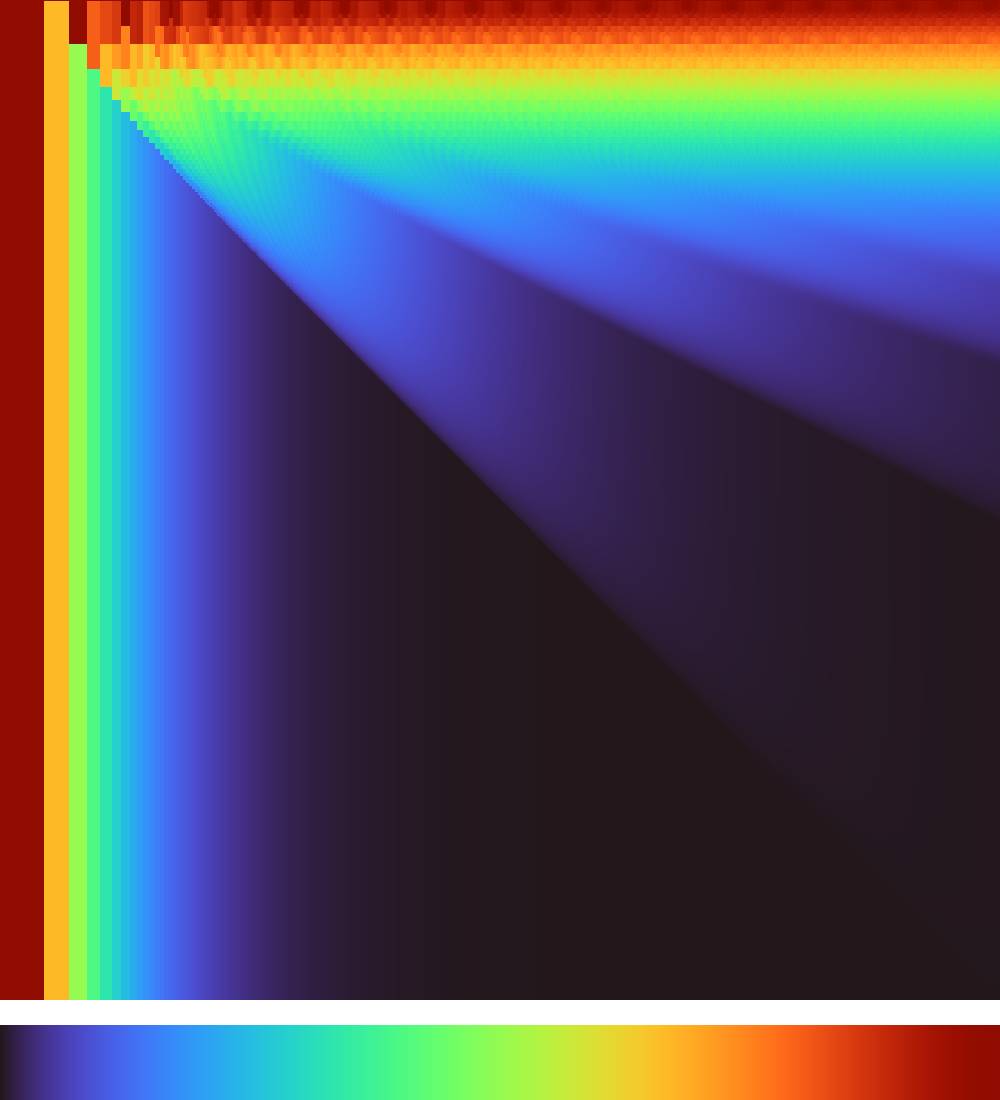
\includegraphics[scale=0.3]{w.png}\,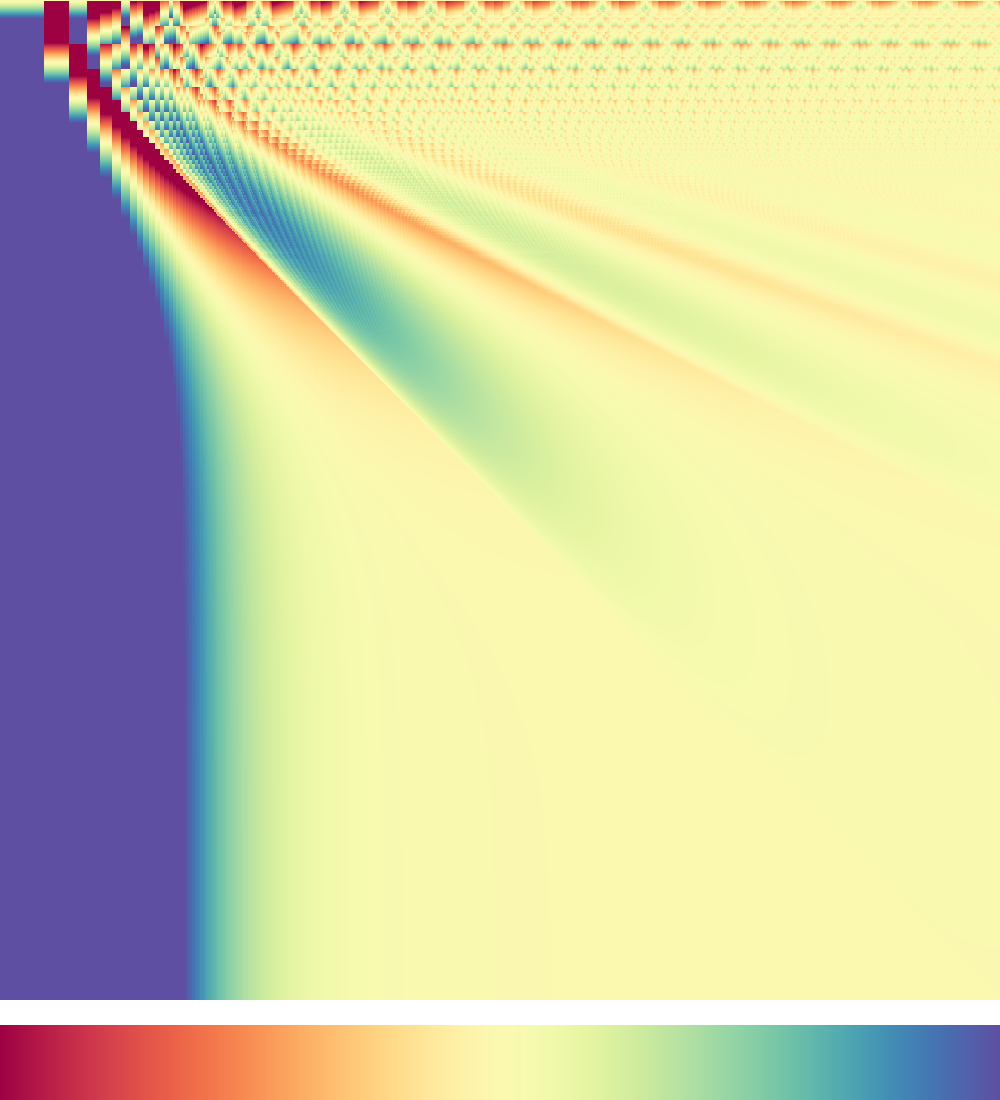
\includegraphics[scale=0.3]{bias.png}
	
	\vspace{0.3cm}
	
	
\includegraphics[scale=0.3]{variance.png}\,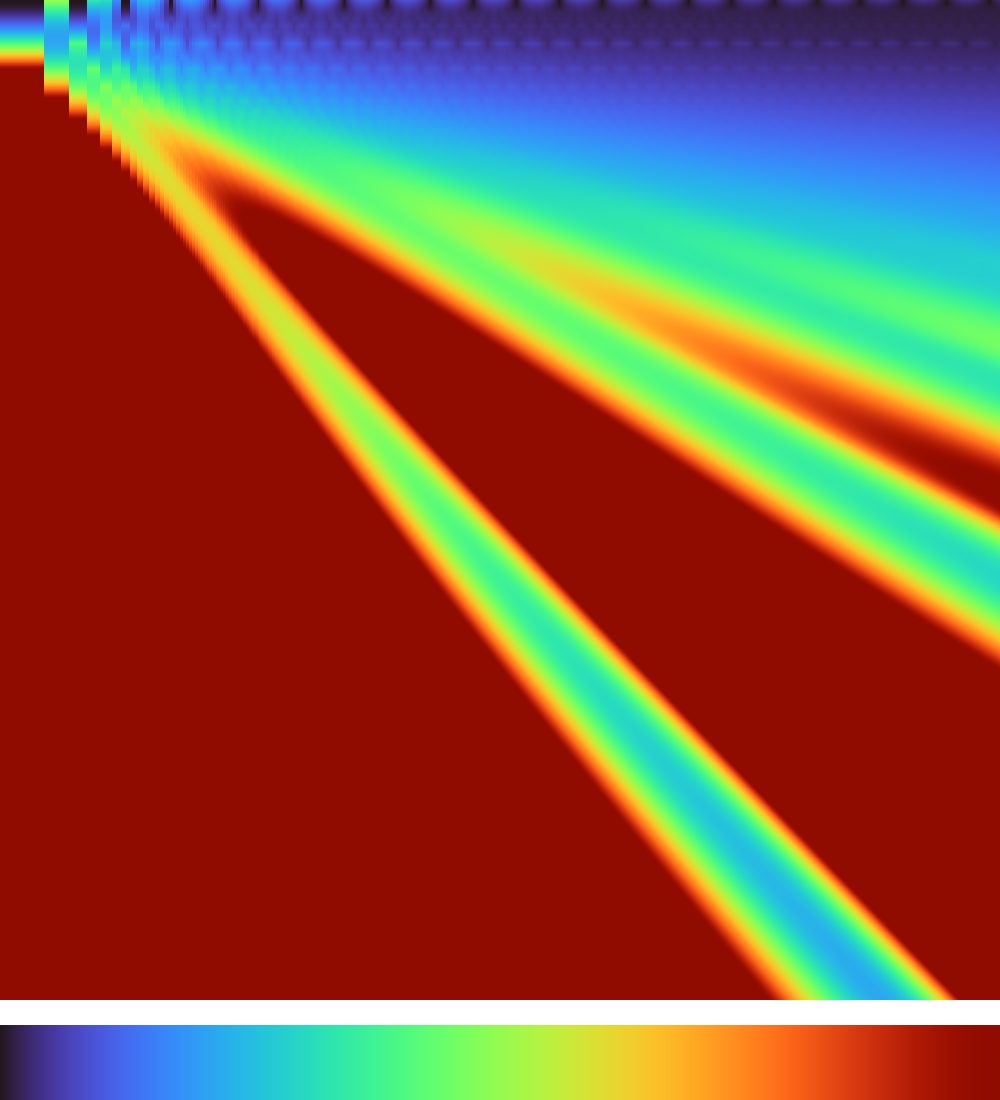
\includegraphics[scale=0.3]{e-bias.png}
	
	\vspace{0.3cm}
	
	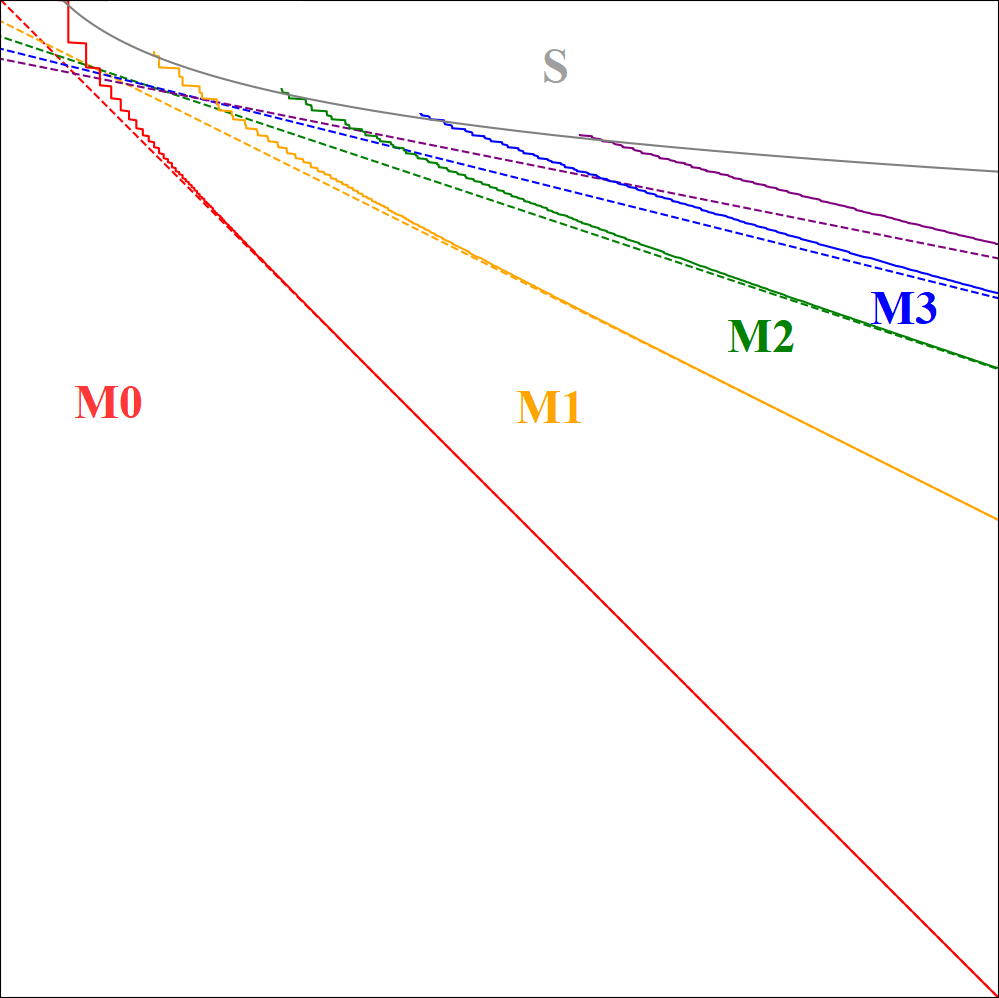
\includegraphics[scale=0.3]{mode.png}
	
	The first graph id colored using the average relative optimizer $w_{s,t}(n)$, where color gradients runs from 0.0 to 0.5
	\[
	c_1 = \frac{w^{\max}_{s,t}(n) + w^{\min}_{s,t}(n)}{2n}
	\]
	The second graph is colored using the relative difference of optimizer $w_{s,t}(n)$ against the continuous optimizer, where 0 difference is light yellow:
	\[
	c_2 = \frac{w^{\max}_{s,t}(n) + w^{\min}_{s,t}(n)}{2n} - g_{s,t}
	\]  
	The third graph is colored using the relative variance of optimizer $w_{s,t}(n)$, where 0 is colored dark green.
	\[
	c_3 = \frac{w^{\max}_{s,t}(n) - w^{\min}_{s,t}(n)}{n}
	\]
	The forth graph is colored using the relative difference between $E(n)$ and its continuous version, where dark blue means little difference, while dark red means $E(n)$ is significantly higher
	\[
	c_4 =\frac{E_{s,t}(n)} {\tilde{E}_{s,t}(n)} = \frac{E_{s,t}(n)} {k_{s,t} n \ln n}
	\]
	
	We can see the graph is divided into several regions. We have already discussed mode $M_0$ and $M_1$ above. There are also mode $M_2$, $M_3$ and so on. A new mode $M_{n+1}$ is formed when the ``short branch" ($E(w)$ when $w$ is small) falls into mode $M_n$. For mode beyond $M_4$, they seems to ``fade away" and becomes very close to the continuous optimizer. We can find the approximated boundaries between these modes. As $t/s$ grows very large, and $g$ becomes very small, we have
	\[
		-\frac{\ln g}{g}\sim \frac{t}{s}
	\]
	\[
		g \sim \frac{W_0(t/s)}{t/s}
	\]
	where $W_0$ is the Lambert W function. We have previously shown that the boundary between $M_0$ and $M_1$ is around
	\[
		n_{0|1}\sim \frac{t}{s}
	\]
	for large $t/s$. Each further mode transition happens when the small branch also encounters a mode transition. The length of the small branch is approximately $w \sim n\cdot g$, so the mode transition point forms geometric sequence approximately
	\[
		n_{k| k+1} \sim n_{k-1| k}/g \sim \left.n_{k-1| k}\middle/\frac{W_0(t/s)}{t/s}\right. \sim \frac{(t/s)^{k+1}}{(W_0(t/s))^{k}}
	\]
	On the logarithmic scale, the boundary between $M_k$ and $M_{k+1}$ looks like a line 
	\[
		\log n_{k| k+1} \sim (k + 1) \log\frac{t}{s} - k\log W_0\left(\frac{t}{s}\right)
	\]
	These lines match what we see in the graphs.
	
	Around $s \approx t$, there is mode $S$.
\end{proof}




\end{document}